% This file makes a web version of the blueprint
% It should include all the \usepackage needed for this version.
% The template includes standard AMS packages.
% It is otherwise a very minimal preamble (you should probably at least
% add cleveref and tikz-cd).

\documentclass{amsbook}

\usepackage{amssymb, amsthm, amsmath}
\usepackage{hyperref}
\usepackage[showmore, dep_graph]{blueprint}
\usepackage{comment}
\usepackage{sagetex}
\usepackage{nicefrac}
\usepackage{tikz-cd}
\usepackage{geometry}
\geometry{verbose,tmargin=1in,bmargin=1in,lmargin=0.5in,rmargin=0.5in}
\usepackage[mathlines]{lineno}

% In this file you should put all LaTeX macros to be used
% both by the pdf version and the web version.
% This should be most of your macros.

% Theorems
\theoremstyle{theorem}
\newtheorem{theorem}{Theorem}[section]%for blueprint
\newtheorem{thm}[theorem]{Theorem}%not for blueprint
\newtheorem{lemma}[theorem]{Lemma}
\newtheorem{lem}[theorem]{Lemma}
\newtheorem{proposition}[theorem]{Proposition}
\newtheorem{prop}[theorem]{Proposition}
\newtheorem{corollary}[theorem]{Corollary}
\newtheorem{cor}[theorem]{Corollary}
\newtheorem{conj}[theorem]{Conjecture}
\newtheorem{rmk}[theorem]{Remark}
\newtheorem{obs}[theorem]{Observation}
\newtheorem{dig}[theorem]{Digression}
\newtheorem{rec}[theorem]{Recall}
\newtheorem{war}[theorem]{Warning}

% Definitions
\theoremstyle{definition}
\newtheorem{definition}[theorem]{Definition}
\newtheorem{defn}[theorem]{Definition}
\newtheorem{example}[theorem]{Example}
\newtheorem{ex}[theorem]{Example}
\newtheorem{nex}[theorem]{Non-Example}
\newtheorem{ntn}[theorem]{Notation}
\newtheorem{con}[theorem]{Convention}

% Number equations in sections
\makeatletter
\let\c@equation\c@theorem
\numberwithin{equation}{section}
\makeatother

\renewcommand\thesection{\thechapter.\arabic{section}}


\renewcommand{\theenumi}{\roman{enumi}}

% Math sets and operators
\newcommand{\Z}{{\mathbb Z}}
\newcommand{\N}{{\mathcal N}}
\newcommand{\K}{{\mathbb K}}
\newcommand{\R}{{\mathbb R}}
\newcommand{\C}{{\mathbb C}}

%enriched (i.e. all large) categories.
\newcommand{\ec}[1]{{\mathord{\mathcal{#1}}}}
\newcommand{\cA}{\ec{A}}
\newcommand{\cC}{\ec{C}}
\newcommand{\cD}{\ec{D}}
\newcommand{\cK}{\ec{K}}
\newcommand{\cL}{\ec{L}}
\newcommand{\cV}{\ec{V}}
\newcommand{\cW}{\ec{W}}
\newcommand{\rQuiv}{\ec{rQuiv}}
\newcommand{\Cat}{\ec{Cat}}
\newcommand{\Kan}{\ec{Kan}}
\newcommand{\qCat}{\ec{QCat}}
\newcommand{\Set}{\ec{Set}}
\newcommand{\sSet}{\ec{sSet}}
\newcommand{\twoCat}{2\text{-}\Cat}
\newcommand{\sCat}{\sSet\text{-}\Cat}
\newcommand{\eCat}[1]{{#1}\text{-}\Cat}%for enriched categories

% Various hom notations.
\newcommand{\qop}[1]{{\mathord{\mathsf{#1}}}}
\newcommand{\Fun}{\qop{Fun}}%mapping spaces in cosmoi
\newcommand{\ho}{\qop{h}}
\newcommand{\hFun}{\qop{hFun}}%hom categories in homotopy 2-categories
\newcommand{\core}{\qop{core}}%not cosmological
\newcommand{\coreop}[1]{{{#1}^\simeq}}%for core as an operator


%1-cells induced from 2-cells
\newcommand{\name}[1]{{\ulcorner{#1}\urcorner}}


% Elementary operators in the theory of (stratified) simplicial sets.

\newcommand{\face}{\delta}
\newcommand{\degen}{\sigma}
\newcommand{\fbv}[1]{\{{#1}\}}


% Duals / Superscripted postfix ops

\newcommand{\op}{^{\mathord{\textup{op}}}}
\newcommand{\co}{^{\mathord{\textup{co}}}}
\newcommand{\coop}{^{\mathord{\textup{coop}}}}

% General operations on maps etc.
\newcommand{\cosk}{\textup{cosk}}
\newcommand{\cod}{\textup{cod}}
\newcommand{\dom}{\textup{dom}}
\newcommand{\ev}{\textup{ev}}
\newcommand{\id}{\textup{id}}
\newcommand{\sk}{\textup{sk}}


%###trial notation for the homotopy 2-category
\newcommand{\h}{\mathfrak{h}}

% Leibniz...
% ... for binary operators like join and product
\newcommand{\leib}[1]{\mathbin{\widehat{#1}}}
% ... for prefix operators like lim, colim and decalage.
\newcommand{\uleib}[1]{\widehat{#1}}
\newcommand{\pwr}{\div}%{\pitchfork}

% In this file you should put macros to be used only by
% the web version. Of course they should have a corresponding
% version in macros/print.tex.
% Typically the printed version could have more fancy decorations.
% This will probably be a very short file.

\newcommand{\coloneq}{:=}

\newcommand{\Del}{\Delta}

\newcommand{\fib}{\twoheadrightarrow}
\newcommand{\we}{\rightsquigarrow}
\newcommand{\trvfib}{\twoheadrightarrow}
\newcommand{\To}{\Rightarrow}%2-cells
\newcommand{\isoto}{\rightsquigarrow}
\newcommand{\inc}{\hookrightarrow}

\newcommand{\catfour}{[3]}
\newcommand{\catthree}{[2]}
\newcommand{\cattwo}{[1]}
\newcommand{\catone}{[0]}
\newcommand{\catn}{[n-1]}
\newcommand{\catnone}{[n]}
\newcommand{\catntwo}{[n+1]}
\newcommand{\iso}{I}



%\github{https://github.com/gnang/Composition-Lemma}


\title{Composition Lemma}
\author{Edinah Gnang}
\author{Parikshit Chalise}

\begin{document}
\linenumbers
\maketitle
\tableofcontents

`% In this file you should put the actual content of the blueprint.
% It will be used both by the web and the print version.
% It should *not* include the \begin{document}
%
% If you want to split the blueprint content into several files then
% the current file can be a simple sequence of \input. Otherwise It
% can start with a \section or \chapter for instance.

\chapter{\texorpdfstring{Composition Lemma}{Composition Lemma}}

\section{Overview}
The \textit{Composition Lemma} was developed and refined over 6 years, beginning in 2018, as a novel approach to settle in the affirmative the \textit{Graceful Tree Conjecture}. The first of such papers was posted in \cite{gnang2020gracefullabelingstrees} by Gnang. A further developed series of papers resolving the same conjecture again appeared in \cite{gnang2022compositionlemma} and \cite{gnang2023proofkotzigringelrosaconjecture}. Recently, the same method has been applied to settle other longstanding conjectures in \cite{chalise2024treenedgesdecomposes} and \cite{chalise2024prooftreepackingconjecture}. We comment that the series of papers shared on the open-source platform arXiv reflect the evolving landscape of Gnang's thought process, and the frequent re-uploads were driven by the natural progression and refinement of ideas. However, we recognize that these numerous edits may have unintentionally caused confusion and raised questions regarding the success of the method. In the current work, we aim to address these concerns by presenting a detailed blueprint of the proof, with the goal of formalizing it in Lean4.



\section{Functional Directed Graphs}\label{sec:Functional Directed Graphs}
For notational convenience, let $\mathbb{Z}_{n}$ denote the set whose members are the first $n$ natural numbers, i.e.,
\begin{equation}
\mathbb{Z}_{n}:=\big\{0,\,1,\ldots,\,n-1\big\}.
\end{equation}
For a function $f:\mathbb{Z}_{m}\to\mathbb{Z}_{n}$, we write $f\in\mathbb{Z}_{n}^{\mathbb{Z}_{m}}$.
For $X\subseteq\mathbb{Z}_{m}$, $f(X)$ denotes the image of $X$
under $f$, i.e.,
\begin{equation}
f(X)=\{f(i):i\in X\},
\end{equation}
and $|f(X)|$ denotes its
cardinality. For $Y\subseteq\mathbb{Z}_{n}\ensuremath{,}f^{-1}(Y)$
denotes the pre-image of $Y$ under $f$ i.e.
\begin{equation}
f^{-1}(Y)=\{j\in\mathbb{Z}_{m}:f(j)\in Y\}
\end{equation}
\begin{definition}[Functional digraphs]\label{defn:functional-directed-graphs}
% REVIEW THE LEAN LABELS BELLOW:
  %\lean{}
  %\leanok
  %\uses{defn:standard-simplex}
For an arbitrary $f\in \mathbb{Z}_n^{\mathbb{Z}_n}$, the \emph{functional directed graph} prescribed by $f$, denoted $G_f$, is such that the vertex set $V(G_f)$ and the directed edge set $E(G_f)$ are respectively as follows:
\[
V(G_f) = \mathbb{Z}_n, \; E(G_f) = \{(v,f(v)):v \in \mathbb{Z}_n\}.
\]
\end{definition}
\begin{definition}[Graceful functional digraphs]\label{defn:graceful-functional-graphs}
  %\lean{}
  %\leanok
  %\uses{defn:functional-directed-graphs}
The functional directed graph prescribed by $f\in\mathbb{Z}_{n}^{\mathbb{Z}_{n}}$ is graceful if there exist
a bijection $\sigma\in \text{S}_n \subset
 \mathbb{Z}_{n}^{\mathbb{Z}_{n}}$ such that
\begin{equation}
\big\{\left|\sigma f\sigma^{-1}(i)-i\right|:i\in\mathbb{Z}_{n}\big\}=\mathbb{Z}_{n}.
\end{equation}
If $\sigma=\text{id}$ (the identity function), then $G_{f}$ --- the functional directed graph prescribed by $f$ --- is gracefully labeled. 
\end{definition}
\begin{defn}[Automorphism group]\label{defn:aut-functional-graphs}
  %\lean{}
  %\leanok
  %\uses{defn:functional-directed-graphs}
For a functional directed graph $G_f$, its automorphism group, denoted $\text{Aut}\left(G_f\right)$, is defined as follows:
\[
\text{Aut}\left(G_f\right) = \large\{\sigma \in \text{S}_n : \{(i, f(i)): i \in \mathbb{Z}_n \} = \{(j, \sigma f \sigma^{-1} (j)) : j \in \mathbb{Z}_n\}\large\}. 
\]
For a polynomial $P \in \mathbb{C}[x_0, \ldots, x_{n-1}]$, its automorphism group, denoted $\text{Aut($P$)}$, is defined as follows:
\[
\text{Aut}\left(P\right)=\large\{\sigma\in\text{S}_{n}:P\left(x_{0},\ldots,x_{i},\ldots,x_{n-1}\right)=P\left(x_{\sigma(0)},\ldots,x_{\sigma(i)},\ldots,x_{\sigma(n-1)}\right)\large\}.
\]
\end{defn}
\begin{definition}[Graceful re-labelings]\label{defn:graceful-functional-graphs-set}
  %\lean{}
  %\leanok
  %\uses{defn:functional-directed-graphs, defn:graceful-functional-graphs}
The set of distinct gracefully labeled functional directed graphs isomorphic to $G_{f}$ is 
\[
\text{GrL}\left(G_{f}\right)\,:=\left\{ G_{\sigma f\sigma^{-1}}:\begin{array}{c}
\sigma\text{ is a representative of a coset in }\nicefrac{\text{S}_{n}}{\text{Aut}\left(G_{f}\right)}\text{ and }\\
\mathbb{Z}_{n}=\left\{ \left|\sigma f\sigma^{-1}\left(i\right)-i\right|\,:\,i\in\mathbb{Z}_{n}\right\} 
\end{array}\right\} 
\]
\end{definition}
\begin{definition}[Complementary labeling involution]\label{defn:complementary-labeling-symmetry}
  %\lean{}
  %\leanok
  %\uses{defn:functional-directed-graphs, defn:graceful-functional-graphs}
If $\varphi=n-1-\text{id}$, i.e. $\varphi \in \mathbb{Z}_{n}^{\mathbb{Z}_{n}}$ such that
\[
\varphi(i)=n-1-i,\, \forall \,i\in \mathbb{Z}_{n},
\]
then for an arbitrary $f\in\mathbb{Z}_{n}^{\mathbb{Z}_{n}}$ the complementary labeling involution is defined as the map
\[
f \mapsto \varphi f \varphi^{-1}
\]
\end{definition}
Observe that for all $f\in \mathbb{Z}_{n}^{\mathbb{Z}_{n}}$ the complementary labeling involution fixes the induced edge label of each edge as seen from the equality
\begin{equation}
\left|f(i)-i\right|=\left|\varphi f(i)-\varphi(i)\right|,\quad\forall\,i\in\mathbb{Z}_{n}.
\end{equation}
In other words, induced edge labels are fixed by the vertex relabeling effected by $\varphi$. We call this induced edge label symmetry the \emph{complementary labeling symmetry} of the functional directed graph $G_f$.


\section{Quotient-Remainder Theorem and Lagrange Interpolation}\label{sec:QRT}
 \begin{proposition}[Multivariate Quotient-Remainder]\label{prop:multivariate-quotient-remainder}
  %\lean{Algebra.Polynomial.FieldDivision}
  %\leanok
  %\uses{}
Let $d(x)\in\mathbb{C}[x]$ be a degree $n$ monic polynomial with
simple roots, i.e.,
\begin{equation}
d(x)=\prod_{u\in\mathbb{Z}_{n}}(x-\alpha_{u})\;\text{ and }\:1=\text{GCD}\big(d(x),\,\frac{d}{dx}d(x)\big),
\end{equation}
where $\{\alpha_{u}:u\in\mathbb{Z}_{n}\}\subset\mathbb{C}$. 
For
all $P\in\mathbb{C}[x_{0},\ldots,x_{m-1}]$, there exists a unique remainder
$r(x_{0},\ldots,x_{m-1})\in\mathbb{C}[x_{0},\ldots,x_{m-1}]$ of degree
at most $n-1$ in each variable such that 
\begin{equation}
P(x_{0},\ldots,x_{m-1})=\sum_{u\in\mathbb{Z}_{m}}q_{u}(x_{0},\ldots,x_{m-1})\,d(x_{u}) \; + \; r(x_{0},\ldots,x_{m-1}).
\end{equation}
 \end{proposition}
\begin{proof}
  %\leanok
We prove by induction on the number of variables that
\begin{equation}
r(x_{0},\ldots,x_{m-1})=\sum_{g\in\mathbb{Z}_{n}^{\mathbb{Z}_{m}}}P(\alpha_{g})\prod_{i\in\mathbb{Z}_{m}}\left(\prod_{j_{i}\in\mathbb{Z}_{n}\backslash\{g(i)\}}\bigg(\frac{x_{i}-\alpha_{j_{i}}}{\alpha_{g(i)}-\alpha_{j_{i}}}\bigg)\right),
\end{equation}
where for notational convenience $P(\alpha_{g}):=P(\alpha_{g(0)},\ldots,\alpha_{g(m-1)})$.
The base case stems from the univariate quotient-remainder theorem over the field $\mathbb{C}$. The univariate-quotient remainder theorem over the field $\mathbb{C}$ asserts that there exit
a unique quotient-remainder pair $\big(q(x_{0}),\,r(x_{0})\big)\in\mathbb{C}[x_{0}]\times\mathbb{C}[x_{0}]$
subject to
\begin{equation}
H(x_{0})=q(x_{0})\,d(x_{0})+r(x_{0}),
\end{equation}
where $r(x_{0})\in\mathbb{C}[x_{0}]$ is of degree at most $n-1$.
It is completely determined by its evaluation over $\{\alpha_{i}:i\in\mathbb{Z}_{n}\}$,
and by Lagrange interpolation we have 
\begin{equation}
r(x_{0})=\sum_{g\in\mathbb{Z}_{n}^{\mathbb{Z}_{1}}}H(\alpha_{g(0)})\prod_{j_{0}\in\mathbb{Z}_{n}\backslash\{g(0)\}}\bigg(\frac{x_{0}-\alpha_{j_{0}}}{\alpha_{g(0)}-\alpha_{j_{0}}}\bigg),
\end{equation}
thus establishing the claim in the base case. For the induction step,
assume as our induction hypothesis that for all $F\in\mathbb{C}\left[x_{0},\ldots,x_{m-1}\right]$,
we have
\begin{equation}
F=\sum_{k\in\mathbb{Z}_{m}}q_{k}(x_{0},\ldots,x_{m-1})\,d(x_{k})+\sum_{g\in\mathbb{Z}_{n}^{\mathbb{Z}_{m}}}F(\alpha_{g})\prod_{i\in\mathbb{Z}_{m}}\left(\prod_{j_{i}\in\mathbb{Z}_{n}\backslash\left\{ g(i)\right\} }\left(\frac{x_{i}-\alpha_{j_{i}}}{\alpha_{g(i)}-\alpha_{j_{i}}}\right)\right).
\end{equation}
We proceed to show that the hypothesis implies that every polynomial in
$m+1$ variables also admits a similar expansion, thus establishing
the desired claim. Consider a polynomial $H \in \mathbb{C}[x_{0},\ldots,x_{m}]$, we view $H$ as a univariate polynomial in the variable $x_{m}$ whose coefficients lie in the field of fraction $\mathbb{C}(x_{0},\ldots,x_{m-1})$.
The univariate quotient-remainder theorem over the field of fractions $\mathbb{C}(x_{0},\ldots,x_{m-1})$ asserts that
there exit a unique quotient-remainder pair
\[
\big(q(x_{m}),\,r(x_{m})\big)\in\big(\mathbb{C}(x_{0},\ldots,x_{m-1})\big)[x_{m}]\times\big(\mathbb{C}(x_{0},\ldots,x_{m-1})\big)[x_{m}]
\]
subject to
\begin{equation}
H\big(x_{0},\ldots,x_{m}\big)=q(x_{0},\ldots,x_{m})\,d(x_{m})+r(x_{0},\ldots,x_{m}),
\end{equation}
where $r\left(x_{0},\ldots,x_{m}\right)\in\big(\mathbb{C}(x_{0},\ldots,x_{m-1})\big)[x_{m}]$
is of degree at most $n-1$ in the variable $x_{m}$. We write 
\begin{equation}
r\left(x_{0},\ldots,x_{m}\right)=\sum_{k\in\mathbb{Z}_{n}}a_{k}\left(x_{0},\ldots,x_{m-1}\right)\,(x_{m})^{k}.
\end{equation}
We now show that coefficients $\big\{ a_k(x_{0},\ldots,x_{m-1}):k\in \mathbb{Z}_n \big\}$ all lie in the polynomial ring $\mathbb{C}[x_{0},\ldots,x_{m-1}]$
via the equality 
\begin{equation}
\bigg(\text{Vander}\left(\begin{array}{c}
\alpha_{0}\\
\vdots\\
\alpha_{u}\\
\vdots\\
\alpha_{n-1}
\end{array}\right)\bigg)\cdot\left(\begin{array}{c}
a_{0}\left(x_{0},\ldots,x_{m-1}\right)\\
\vdots\\
a_{u}\left(x_{0},\ldots,x_{m-1}\right)\\
\vdots\\
a_{n-1}\left(x_{0},\ldots,x_{m-1}\right)
\end{array}\right)=\left(\begin{array}{c}
H(x_{0},\ldots,x_{m-1},\alpha_{0})\\
\vdots\\
H(x_{0},\ldots,x_{m-1},\alpha_{u})\\
\vdots\\
H(x_{0},\ldots,x_{m-1},\alpha_{n-1})
\end{array}\right),
\end{equation}
where 
\begin{equation}
\bigg(\text{Vander}\left(\begin{array}{c}
\alpha_{0}\\
\vdots\\
\alpha_{u}\\
\vdots\\
\alpha_{u}
\end{array}\right)\bigg)\left[i,j\right]=(\alpha_{i})^{j},\ \forall\,0\le i,j<n.
\end{equation}
Since the Vandermonde matrix is invertible by the fact
\begin{equation}
0\ne\det\bigg(\text{Vander}\left(\begin{array}{c}
\alpha_{0}\\
\vdots\\
\alpha_{u}\\
\vdots\\
\alpha_{u}
\end{array}\right)\bigg)=\prod_{0\le u<v<n}(\alpha_{v}-\alpha_{u}),
 \end{equation}
we indeed have 
\begin{equation}
\left(\begin{array}{c}
a_{0}\left(x_{0},\ldots,x_{m-1}\right)\\
\vdots\\
a_{u}\left(x_{0},\ldots,x_{m-1}\right)\\
\vdots\\
a_{n-1}\left(x_{0},\ldots,x_{m-1}\right)
\end{array}\right)=\bigg(\text{Vander}\left(\begin{array}{c}
\alpha_{0}\\
\vdots\\
\alpha_{u}\\
\vdots\\
\alpha_{u}
\end{array}\right)\bigg)^{-1}\cdot\left(\begin{array}{c}
H(x_{0},\ldots,x_{m-1},\alpha_{0})\\
\vdots\\
H(x_{0},\ldots,x_{m-1},\alpha_{u})\\
\vdots\\
H(x_{0},\ldots,x_{m-1},\alpha_{n-1})
\end{array}\right).
\end{equation}
Therefore, we have 
\begin{equation}
H\big(x_{0},\ldots,x_{m}\big)
= q_{m}\big(x_{0},\ldots,x_{m}\big)\,d(x_{m})+\sum_{g(m)\in\mathbb{Z}_{n}}H\big(x_{0},\ldots,x_{m-1},\alpha_{g(m)}\big)\prod_{j\in\mathbb{Z}_{n}\backslash\{g(m)\}}\left(\frac{x_{m}-\alpha_{j_{m}}}{\alpha_{g(m)}-\alpha_{j_{m}}}\right).
\end{equation}
Applying the induction hypothesis to coefficients
\[
\left\{ H\left(x_{0},\ldots,x_{m-1},g\left(m\right)\right):g\left(m\right)\in\mathbb{Z}_{n}\right\} \subset\mathbb{C}[x_{0},\ldots,x_{m-1}]
\]
yields the desired claim.
\end{proof}
 \begin{proposition}[Ring Homomorphism]\label{prop:ring-homomorphism}
  %\lean{Algebra.Polynomial.FieldDivision}
  %\leanok
  %\uses{}
For an arbitrary $H\in\mathbb{C}\left[x_{0},\ldots,x_{n-1}\right]$, let $\overline{H}$ denote
the {remainder} of the congruence class 
\[
H\mod\left\{ d(x_{i}):i\in\mathbb{Z}_{n}\right\} ,
\]
where
\[
d(x)=\prod_{u\in\mathbb{Z}_{n}}(x-\alpha_{u})\;\text{ and }\:1=\text{GCD}\big(d(x),\,\frac{d}{dx}d(x)\big),
\]
Then the following hold:
\begin{enumerate}
    \item Evaluations over the  lattice $\{\alpha_{u}:u\in\mathbb{Z}_{n}\}^{n}$ of $\overline{H}$ match evaluations of $H$ over the same lattice. 
    \item If $H = H_1 + H_2,$ where $H_1, H_2 \in \mathbb{C}\left[x_{0},\ldots,x_{n-1}\right]$, then $\overline{H_1} + \overline{H_2} = \overline{H}$.
\end{enumerate}
 \end{proposition}
\begin{proof}
  %\leanok
  The first claim follows from Proposition \ref{prop:multivariate-quotient-remainder} for we see that the quotient divisor part vanishes over the lattice. To prove the second claim we recall that
  \[
\overline{H}=\sum_{g\in\mathbb{Z}_{n}^{\mathbb{Z}_{m}}}H(\alpha_{g})\prod_{i\in\mathbb{Z}_{m}}\left(\prod_{j_{i}\in\mathbb{Z}_{n}\backslash\{g(i)\}}\bigg(\frac{x_{i}-\alpha_{j_{i}}}{\alpha_{g(i)}-\alpha_{j_{i}}}\bigg)\right),
  \]
  \[
  \implies\overline{H}=\sum_{g\in\mathbb{Z}_{n}^{\mathbb{Z}_{m}}}\big(H_{1}(\alpha_{g})+H_{2}(\alpha_{g})\big)\prod_{i\in\mathbb{Z}_{m}}\left(\prod_{j_{i}\in\mathbb{Z}_{n}\backslash\{g(i)\}}\bigg(\frac{x_{i}-\alpha_{j_{i}}}{\alpha_{g(i)}-\alpha_{j_{i}}}\bigg)\right),
  \]
  \[
  \implies\overline{H}=\sum_{k\in\{1,2\}}\sum_{g\in\mathbb{Z}_{n}^{\mathbb{Z}_{m}}}H_{k}(\alpha_{g})\prod_{i\in\mathbb{Z}_{m}}\left(\prod_{j_{i}\in\mathbb{Z}_{n}\backslash\{g(i)\}}\bigg(\frac{x_{i}-\alpha_{j_{i}}}{\alpha_{g(i)}-\alpha_{j_{i}}}\bigg)\right).
  \]
  Thus $\overline{H_1} + \overline{H_2} = \overline{H}$ as claimed.
\end{proof}
\begin{defn}[Polynomial of Grace]\label{defn:polynomial-grace-definition} We define $P_f \in \mathbb{C}[x_0, \ldots, x_{n-1}]$ for all $f \in \mathbb{Z}_n^{\mathbb{Z}_n}$ as follows:
\begin{equation}
    P_f \coloneq \underbrace{\prod_{0\le u<v<n}(x_{v}-x_{u})}_{V(x_0,\ldots,x_{n-1})}\,\underbrace{\prod_{0\le u<v<n}\big((x_{f(v)}-x_{v})^{2}-(x_{f(u)}-x_{u})^{2}\big)}_{E_f(x_0,\ldots,x_{n-1})}.
\end{equation}
\end{defn}
\begin{defn}[Congruence class]\label{defn:polynomial-congruence}
  %\lean{}
  %\leanok
  %\uses{prop:multivariate-quotient-remainder}
For polynomials $P,Q \in \mathbb{C}[x_0, \ldots, x_{n-1}]$, if
\begin{equation}
P({\bf x}) \equiv \; Q({\bf x}) \; \mod\bigg\{\prod_{j\in\mathbb{Z}_{n}}(x_{i}-j):i\in\mathbb{Z}_{n}\bigg\},
\end{equation}
we simply write $P \equiv Q$.
\end{defn}
 Unless otherwise stated, all congruence relations in this paper are prescribed modulo the ideal of polynomials generated by members of the set
\[
\bigg\{\prod_{j\in\mathbb{Z}_{n}}(x_{i}-j):i\in\mathbb{Z}_{n}\bigg\}
\]
\begin{proposition}[Certificate of Grace]\label{prop:polynomial-grace-certificate}
  %\lean{}
  %\leanok
  %\uses{defn:polynomial-grace-definition, defn:polynomial-congruence, prop:multivariate-quotient-remainder}
Let $f\in\mathbb{Z}_{n}^{\mathbb{Z}_{n}}$. The functional
directed graph $G_f$ prescribed by $f$ is graceful if and only if $P_f(\mathbf{x}) \; \not\equiv \; 0$.
\end{proposition}
\begin{proof}
Observe that the vertex Vandermonde factor $V(\mathbf{x})$ is of degree exactly $n-1$ in each variable and therefore equal
to its remainder, i.e.,
\begin{equation}\label{eq:Vf}
V(\mathbf{x})=\sum_{\theta\in\text{S}_{n}}\text{sgn}(\theta)\prod_{i\in\mathbb{Z}_{n}}(x_{i})^{\theta(i)}=\prod_{v\in\mathbb{Z}_{n}}v!\;\sum_{\theta\in\text{S}_{n}}\text{sgn}(\theta)\prod_{\begin{array}{c}
\substack{i\in\mathbb{Z}_{n}\\
j_{i}\in\mathbb{Z}_{n}\backslash\{\theta(i)\}
}
\end{array}}\left(\frac{x_{i}-j_{i}}{\theta(i)-j_{i}}\right),
\end{equation}
where 
\begin{equation}
\text{sgn}(\theta):=\prod_{0\le u<v<n}\left(\frac{\theta(v)-\theta(u)}{v-u}\right),\quad\forall\,\theta\in\text{S}_{n}.
\end{equation}
The induced edge label Vandermonde factor $E_f(\mathbf{x})$
is of degree $>n-1$ in some of its variables. Therefore, by Proposition  \ref{prop:multivariate-quotient-remainder}, we have
\begin{equation}\label{eq:Ef}
E_{f}(\mathbf{x})=\sum_{l\in\mathbb{Z}_{m}}q_{l}(\mathbf{x})\prod_{k\in\mathbb{Z}_{n}}(x_{l}-k)+\sum_{g\in\mathbb{Z}_{n}^{\mathbb{Z}_{n}}}\,\prod_{0\le u<v<n}\left(\big(gf(v)-g(v)\big)^{2}-\big(gf(u)-g(u)\big)^{2}\right)\prod_{\begin{array}{c}
\substack{i\in\mathbb{Z}_{n}\\
j_{i}\in\mathbb{Z}_{n}\backslash\{g(i)\}
}
\end{array}}\left(\frac{x_{i}-j_{i}}{g(i)-j_{i}}\right).
\end{equation}
Observe that by the expansions in \ref{eq:Vf} and \ref{eq:Ef}, 
\[
P_f(\mathbf{x})=\sum_{l\in\mathbb{Z}_{m}}q_{l}(\mathbf{x})V(\mathbf{x})\prod_{k\in\mathbb{Z}_{n}}(x_{l}-k)+
\]
\[
\left(\prod_{v\in\mathbb{Z}_{n}}v!\sum_{\theta\in\text{S}_{n}}\text{sgn}(\theta)\prod_{\begin{array}{c}
\substack{i\in\mathbb{Z}_{n}\\
j_{i}\in\mathbb{Z}_{n}\backslash\{\theta(i)\}
}
\end{array}}\left(\frac{x_{i}-j_{i}}{\theta(i)-j_{i}}\right)\right)\left(\sum_{g\in\mathbb{Z}_{n}^{\mathbb{Z}_{n}}}\prod_{0\le u<v<n}\bigg(\big(gf(v)-g(v)\big)^{2}-\big(gf(u)-g(u)\big)^{2}\bigg)\prod_{\begin{array}{c}
\substack{i\in\mathbb{Z}_{n}\\
j_{i}\in\mathbb{Z}_{n}\backslash\{g(i)\}
}
\end{array}}\left(\frac{x_{i}-j_{i}}{g(i)-j_{i}}\right)\right).
\]
is congruent to
\begin{equation} \label{eq:graceful-evaluation}
\prod_{v\in\mathbb{Z}_{n}}\left(v!\right)^{2}\frac{\left(n-1+v\right)!}{\left(2v\right)!}\sum_{\begin{array}{c}
\substack{\sigma\in\text{S}_{n}\\
\gamma=\left|\sigma f\sigma^{-1}-\text{id}\right|\in\text{S}_{n}
}
\end{array}}\text{sgn}(\gamma\sigma)\prod_{\begin{array}{c}
\substack{i\in\mathbb{Z}_{n}\\
j_{i}\in\mathbb{Z}_{n}\backslash\{\sigma(i)\}
}
\end{array}}\left(\frac{x_{i}-j_{i}}{\sigma(i)-j_{i}}\right), 
\end{equation}
where the permutation $\gamma$ denotes the induced edge label permutation associated with a graceful relabeling $G_{\sigma f\sigma^{-1}}$ of $G_f$.
The congruence above stems from the congruence identity
\[
\prod_{\begin{array}{c}
\substack{i\in\mathbb{Z}_{n}\\
j_{i}\in\mathbb{Z}_{n}\backslash\{\theta(i)\}
}
\end{array}}\left(\frac{x_{i}-j_{i}}{\theta(i)-j_{i}}\right)\prod_{\begin{array}{c}
\substack{i\in\mathbb{Z}_{n}\\
j_{i}\in\mathbb{Z}_{n}\backslash\{g(i)\}
}
\end{array}}\left(\frac{x_{i}-j_{i}}{g(i)-j_{i}}\right)\equiv\begin{cases}
\begin{array}{cc}
\underset{\begin{array}{c}
\substack{i\in\mathbb{Z}_{n}\\
j_{i}\in\mathbb{Z}_{n}\backslash\{\theta(i)\}
}
\end{array}}{\prod}\left(\frac{x_{i}-j_{i}}{\theta(i)-j_{i}}\right) & \text{ if }\theta=g\\
\\0 & \text{otherwise}
\end{array} & \forall\,(\theta,g)\in\text{S}_{n}\times\mathbb{Z}_{n}^{\mathbb{Z}_{n}}\end{cases}
\]
and a graceful labeling necessitates the integer coefficient
\[
\prod_{0\le i<j<n}(j-i)\big(j^{2}-i^{2})=\prod_{0\le i<j<n}(j-i)^{2}(j+i)=\prod_{v\in\mathbb{Z}_{n}}\left(v!\right)^{2}\frac{\left(n-1+v\right)!}{\left(2v\right)!} \neq 0,
\]
thus establishing the desired claim.
\end{proof}
\begin{example} We present an example of a path on 5 vertices. This is known to be graceful, so we expect a non-zero remainder.
\ \\
\begin{center}   
\resizebox{!}{3em}{
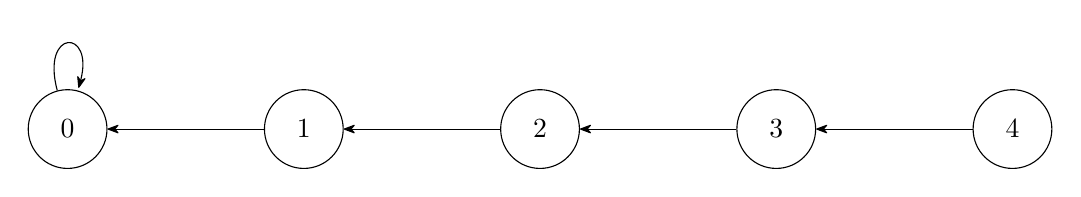
\begin{tikzpicture}[>={Stealth[round]}, node distance=2cm and 1cm, every node/.style={circle, draw, minimum size=1cm}]
    % Define vertices
    \node (v0) at (0, 0) {0};
    \node (v1) at (3, 0) {1};
    \node (v2) at (6, 0) {2};
    \node (v3) at (9, 0) {3};
    \node (v4) at (12, 0) {4};
    
    % Draw edges
    \draw [->] (v1) to (v0); % Edge 1 -> 0
    \draw [->] (v2) to (v1); % Edge 2 -> 1
    \draw [->] (v3) to (v2); % Edge 3 -> 2
    \draw [->] (v4) to (v3); % Edge 4 -> 3
    \draw[->] (v0) edge[loop above] (v0); % Self-loop at 0
\end{tikzpicture}
}
\end{center}
Run the SageMath script \texttt{ex1325.sage} to verify.
\end{example}
\begin{proposition}[Complementary Labeling Symmetry]\label{prop:complementary-labeling-Symmetry}
%\lean{}
  %\leanok
  %\uses{defn:graceful-functional-graphs, defn:graceful-functional-graphs-set, prop:multivariate-quotient-remainder, defn:polynomial-grace-definition, defn:polynomial-congruence, prop:polynomial-grace-certificate, prop:complementary-labeling-Symmetry}
Let $f\in\mathbb{Z}_{n}^{\mathbb{Z}_{n}}$ and the remainder of $P_f$ be
\begin{equation}
\overline{P}_f(\mathbf{x}):=\prod_{v\in\mathbb{Z}_{n}}\left(v!\right)^{2}\frac{\left(n-1+v\right)!}{\left(2v\right)!}\sum_{\begin{array}{c}
\substack{\sigma\in\text{S}_{n}\\
\gamma=\left|\sigma f\sigma^{-1}-\text{id}\right|\in\text{S}_{n}
}
\end{array}}\text{sgn}(\gamma\sigma)\prod_{\begin{array}{c}
\substack{i\in\mathbb{Z}_{n}\\
j_{i}\in\mathbb{Z}_{n}\backslash\{\sigma(i)\}
}
\end{array}}\left(\frac{x_{i}-j_{i}}{\sigma(i)-j_{i}}\right). 
\end{equation}
The complementary labeling map $x_{i}\mapsto x_{n-1-i},$ for all $i\in \mathbb{Z}_n$,
fixes $\overline{P}_f$ up to sign.
\end{proposition}
\begin{proof}
For notational convenience, let $\mathbf{x}_{\varphi}:=x_{\varphi(0)},\ldots,x_{\varphi(i)},\ldots,x_{\varphi(n-1)}$. Observe that for any permutation $\varphi\in \text{S}_n$, the action of $\varphi$ on $P_f$ yields equalities
 \[
 \begin{array}{ccc}
P_{f}({\bf x}_{\varphi}) & = & \underset{0\le u<v<n}{\prod}(x_{\varphi(v)}-x_{\varphi(u)})\big((x_{\varphi f(v)}-x_{\varphi(v)})^{2}-(x_{\varphi f(u)}-x_{\varphi(u)})^{2}\big),\\
\\
 & = & \underset{0\le\varphi^{-1}(i)<\varphi^{-1}(j)<n}{\prod}(x_{j}-x_{i})\big((x_{\varphi f\varphi^{-1}(j)}-x_{j})^{2}-(x_{\varphi f\varphi^{-1}(i)}-x_{i})^{2}\big).
\end{array}
 \]
 The last equality above features the indexing change of variable $u=\varphi^{-1}(i)$ and $v=\varphi^{-1}(j)$. Thus, $P_{f}(x_{\varphi(0)},\ldots,x_{\varphi(n-1)})$ is up to sign equal to $P_{\varphi f\varphi^{-1}}$, in accordance with Definition \ref{defn:polynomial-grace-definition}. Furthermore, by the proof of Proposition \ref{prop:polynomial-grace-certificate}, the action of $\varphi$
on $P_{f}$ yields the congruence identity
\[
P_{f}(\mathbf{x}_{\varphi})\equiv \overline{P}_f(\mathbf{x}_{\varphi}).
\]
Hence,
\begin{align*}
    \overline{P}_f({\bf x}_{\varphi})	& =\prod_{v\in\mathbb{Z}_{n}}\bigg(\left(v!\right)^{2}\frac{\left(n-1+v\right)!}{\left(2v\right)!}\bigg)\sum_{\substack{\sigma\in\text{S}_{n}\\
\gamma=\left|\sigma f\sigma^{-1}-\text{id}\right|\in\text{S}_{n}
}
}\text{sgn}(\gamma\sigma)\prod_{\substack{i\in\mathbb{Z}_{n}\\
j_{i}\in\mathbb{Z}_{n}\backslash\{\sigma(i)\}
}
}\bigg(\frac{x_{\varphi(i)}-j_{i}}{\sigma(i)-j_{i}}\bigg),\\
	&=\text{sgn}(\varphi)\prod_{v\in\mathbb{Z}_{n}}\bigg(\left(v!\right)^{2}\frac{\left(n-1+v\right)!}{\left(2v\right)!}\bigg)\sum_{\substack{\sigma\in\text{S}_{n}\\
\gamma=\left|\sigma f\sigma^{-1}-\text{id}\right|\in\text{S}_{n}
}
}\text{sgn}(\gamma\sigma\varphi^{-1})\prod_{\substack{u\in\mathbb{Z}_{n}\\
v_{u}\in\mathbb{Z}_{n}\backslash\{\sigma\varphi^{-1}(u)\}
}
}\bigg(\frac{x_{u}-v_{u}}{\sigma\varphi^{-1}(u)-v_{u}}\bigg).
\end{align*}
If $\varphi=n-1-\text{id}$, then,
by the complementary labeling symmetry, we have 
\[
G_{\sigma f\sigma^{-1}}\in\text{GrL}\left(G_{f}\right)\Longleftrightarrow G_{\sigma\varphi^{-1}f(\sigma\varphi^{-1})^{-1}}\in\text{GrL}\left(G_{f}\right)
\]
Let $\mathfrak{G}$ denote the subrgoup of $\text{S}_n$ whose members are $\big\{\text{id},\ \varphi\big\}$. We write
\[
\overline{P}_f(\mathbf{x}_\varphi)=
\]
\[
\prod_{v\in\mathbb{Z}_{n}}\bigg(\left(v!\right)^{2}\frac{\left(n-1+v\right)!}{\left(2v\right)!}\bigg)\sum_{\begin{array}{c}
\substack{\sigma\in\nicefrac{\text{S}_{n}}{\mathfrak{G}}\\
\gamma=\left|\sigma f\sigma^{-1}-\text{id}\right|\in\text{S}_{n}
}
\end{array}}\text{sgn}(\gamma\sigma)\left(\text{sgn}(\varphi^{-1})\prod_{\substack{u\in\mathbb{Z}_{n}\\
v_{u}\in\mathbb{Z}_{n}\backslash\{\sigma(u)\}
}
}\bigg(\frac{x_{u}-v_{u}}{\sigma(u)-v_{u}}\bigg)+\prod_{\substack{u\in\mathbb{Z}_{n}\\
v_{u}\in\mathbb{Z}_{n}\backslash\{\sigma\varphi^{-1}(u)\}
}
}\bigg(\frac{x_{u}-v_{u}}{\sigma\varphi^{-1}(u)-v_{u}}\bigg)\right).
\]
Similarly, 
\[
\overline{P}_f(\mathbf{x})=
\]
\[
\prod_{v\in\mathbb{Z}_{n}}\bigg(\left(v!\right)^{2}\frac{\left(n-1+v\right)!}{\left(2v\right)!}\bigg)\sum_{\begin{array}{c}
\substack{\sigma\in\nicefrac{\text{S}_{n}}{\mathfrak{G}}\\
\gamma=\left|\sigma f\sigma^{-1}-\text{id}\right|\in\text{S}_{n}
}
\end{array}}\text{sgn}(\gamma\sigma)\left(\prod_{\begin{array}{c}
\substack{i\in\mathbb{Z}_{n}\\
j_{i}\in\mathbb{Z}_{n}\backslash\{\sigma(i)\}
}
\end{array}}\bigg(\frac{x_{i}-j_{i}}{\sigma(i)-j_{i}}\bigg)+\text{sgn}(\varphi^{-1})\prod_{\begin{array}{c}
\substack{i\in\mathbb{Z}_{n}\\
j_{i}\in\mathbb{Z}_{n}\backslash\{\sigma\varphi^{-1}(i)\}
}
\end{array}}\bigg(\frac{x_{i}-j_{i}}{\sigma\varphi^{-1}(i)-j_{i}}\bigg)\right).
\]
We conclude that the complementary labeling symmetry yields the equality
\[
\overline{P}_f(\mathbf{x})=\text{sgn}(\varphi)\,\overline{P}_f(\mathbf{x}_{\varphi})=\overline{P}_{\varphi f\varphi^{-1}}(\mathbf{x}),
\]
thus establishing the desired claim.
\end{proof}

\begin{example} We present an example of a path on 5 vertices.
\ \\
\begin{center}   
\resizebox{!}{3em}{
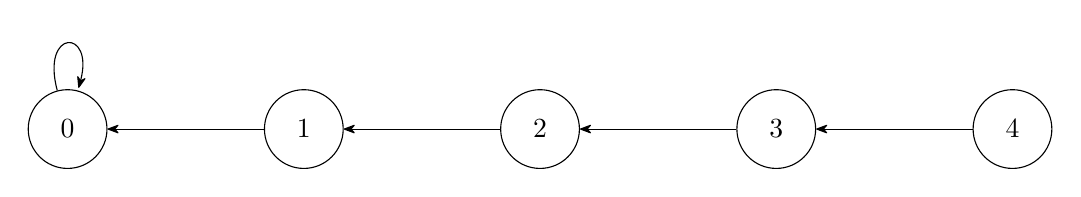
\begin{tikzpicture}[>={Stealth[round]}, node distance=2cm and 1cm, every node/.style={circle, draw, minimum size=1cm}]
    % Define vertices
    \node (v0) at (0, 0) {0};
    \node (v1) at (3, 0) {1};
    \node (v2) at (6, 0) {2};
    \node (v3) at (9, 0) {3};
    \node (v4) at (12, 0) {4};
    
    % Draw edges
    \draw [->] (v1) to (v0); % Edge 1 -> 0
    \draw [->] (v2) to (v1); % Edge 2 -> 1
    \draw [->] (v3) to (v2); % Edge 3 -> 2
    \draw [->] (v4) to (v3); % Edge 4 -> 3
    \draw[->] (v0) edge[loop above] (v0); % Self-loop at 0
\end{tikzpicture}
}
\end{center}
Run the SageMath script \texttt{ex1328.sage} to verify.
\end{example}

\begin{lemma}[Variable Dependency] \label{lem:variable-dependency}
  %\lean{}
  %\leanok
  %\uses{prop:multivariate-quotient-remainder}
Let $P\in\mathbb{Q}\left[x_{0},\ldots,x_{n-1}\right]$
and $S\subsetneq\mathbb{Z}_{n}$. If 
\begin{equation}
P(\mathbf{x})=\sum_{g\in\mathbb{Z}_{n}^{S}}c_{g}\,\prod_{i\in S}(x_{i})^{g(i)},
\end{equation}
where $c_g \in\mathbb{C}$ for all $g\in\mathbb{Z}_{n}^{S}$, then for any positive integer $m$, the polynomial $\big(P(\mathbf{x})\big)^{m}$
admits a quotient-remainder expansion of the form
\begin{equation}
\big(P(x_0,\ldots,x_{n-1})\big)^{m}=\sum_{j\in\mathbb{Z}_{m}}q_{j}(x_0,\ldots,x_{n-1})\prod_{k\in\mathbb{Z}_{n}}(x_{j}-\alpha_{k})+\sum_{g\in\mathbb{Z}_{n}^{S}}a_{g}\prod_{i\in S}(x_{i})^{g(i)}
\end{equation}
where $\alpha_k, a_g\in \mathbb{C}$ for all $k\in \mathbb{Z}_n$ such that $n=\left|\big\{\alpha_{k}:k\in\mathbb{Z}_{n}\big\}\right|$and $g\in\mathbb{Z}_{n}^{S}$.
\end{lemma}

\begin{proof}
  %\leanok
  By the premise, the polynomial $P({\bf x})$ is of degree at most $n-1$
in its variables. Thus by Proposition \ref{prop:multivariate-quotient-remainder}, the polynomial $P({\bf x})$
is equal to its remainder, i.e.,
\begin{equation}
P(\mathbf{x})\;=\;\sum_{g\in\mathbb{Z}_{n}^{S}}c_{g}\,\prod_{i\in S}(x_{i})^{g(i)}\;=\;\sum_{g\in\mathbb{Z}_{n}^{S}}P(g)\prod_{\begin{array}{c}
\substack{i\in S\\
j_{i}\in\mathbb{Z}_{n}\backslash\left\{ g(i)\right\} 
}
\end{array}}\left(\frac{x_{i}-\alpha_{j_{i}}}{\alpha_{g(i)}-\alpha_{j_{i}}}\right).
\end{equation}
 The remainder of $(P({\bf x}))^m$ is obtained by repeatedly replacing each occurrence
of $(x_{i})^{n}$ with $(x_{i})^{n}-\underset{k\in\mathbb{Z}_{n}}{\prod}(x_{i}-\alpha_{k})$, followed by expanding the resulting polynomials, starting from the
expanded form of 
\begin{equation}
\bigg(\sum_{g\in\mathbb{Z}_{n}^{S}}c_{g}\,\prod_{i\in S}(x_{i})^{g(i)}\bigg)^{m},
\end{equation}
until we obtain a polynomial of degree at most $n-1$ in each variable.
The transformation never introduces a variable indexed by a member
of the complement of $S$. We obtain that 
\[
\bigg(\sum_{g\in\mathbb{Z}_{n}^{S}}c_{g}\,\prod_{i\in S}(x_{i})^{g(i)}\bigg)^{m}=\sum_{j\in\mathbb{Z}_{m}}q_{j}(\mathbf{x})\prod_{k\in\mathbb{Z}_{n}}(x_{j}-\alpha_{k})+\sum_{g\in\mathbb{Z}_{n}^{S}}\big(P(g)\big)^{m}\prod_{\begin{array}{c}
\substack{i\in S\\
j_{i}\in\mathbb{Z}_{n}\backslash\left\{ g(i)\right\} 
}
\end{array}}\left(\frac{x_{i}-\alpha_{j_{i}}}{\alpha_{g(i)}-\alpha_{j_{i}}}\right)
\]
by which it follows that 
\begin{equation}
\bigg(\sum_{g\in\mathbb{Z}_{n}^{S}}c_{g}\,\prod_{i\in S}(x_{i})^{g(i)}\bigg)^{m}=\sum_{j\in\mathbb{Z}_{m}}q_{j}(\mathbf{x})\prod_{k\in\mathbb{Z}_{n}}(x_{j}-\alpha_{k})+\sum_{g\in\mathbb{Z}_{n}^{S}}a_{g}\prod_{i\in S}(x_{i})^{g(i)},
\end{equation}
where $\alpha_k, a_g\in \mathbb{C}$ for all $k\in \mathbb{Z}_n$ and $n=\left|\big\{\alpha_{k}:k\in\mathbb{Z}_{n}\big\}\right|$
as claimed.
\end{proof}
\begin{lemma} [Monomial support] \label{lem:monomial-support}
  %\lean{}
  %\leanok
  %\uses{prop:multivariate-quotient-remainder}
 Let $P\in\mathbb{Q}[x_{0},\ldots,x_{n-1}]$ be such that it is not identically
constant. If 
\begin{equation}
P(\mathbf{x})\;=\;\sum_{\sigma\in\text{S}_{n}}a_{\sigma}\prod_{\begin{array}{c}
\substack{i\in\mathbb{Z}_{n}\\
j_{i}\in\mathbb{Z}_{n}\backslash\{\sigma(i)\}
}
\end{array}}\left(\frac{x_{i}-j_{i}}{\sigma(i)-j_{i}}\right),
\end{equation}
then there exist a minimal non-empty set $\mathcal{M}_{P}\subset\mathbb{Z}_{n}^{\mathbb{Z}_{n}}$
subject to $\left|f^{-1}\left(\left\{ 0\right\} \right)\right|\le1$
for all $f\in\mathcal{M}_{P}$ such that 
\begin{equation}
P(\mathbf{x})=\sum_{f\in\mathcal{M}_{P}}c_{f}\prod_{i\in\mathbb{Z}_{n}}x_{i}^{f\left(i\right)},
\end{equation}
where $c_{f}\in\mathbb{Q}\setminus\{0\}$.
\end{lemma}
\begin{proof}
  %\leanok
  Stated otherwise, every term in the expanded form of $P$ is
a multiple of at least $n-1$ distinct variables. Consider a Lagrange
basis polynomial associated with an arbitrary $\sigma\in\text{S}_{n}$:
\[
L_{\sigma}({\bf x})=\prod_{\substack{i\in\mathbb{Z}_{n}\\
j_{i}\in\mathbb{Z}_{n}\setminus\{\sigma(i)\}
}
}\bigg(\frac{x_{i}-j_{i}}{\sigma(i)-j_{i}}\bigg)\;=\;\prod_{\begin{array}{c}
\substack{i\in\mathbb{Z}_{n}\setminus\{\sigma^{-1}(0)\}\\
j_{i}\in\mathbb{Z}_{n}\backslash\{\sigma(i)\}
}
\end{array}}\left(\frac{x_{i}-j_{i}}{\sigma\left(i\right)-j_{i}}\right)\prod_{j_{\sigma^{-1}\left(0\right)}\in\mathbb{Z}_{n}\backslash\left\{ 0\right\} }\left(\frac{x_{\sigma^{-1}\left(0\right)}-j_{\sigma^{-1}\left(0\right)}}{0-j_{\sigma^{-1}\left(0\right)}}\right).
\]
On the right-hand side of the second equal sign immediately above,
the univariate polynomial in $x_{\sigma^{-1}(0)}$ encompassed within the scope of the second $\Pi$
indexed by $j_{\sigma^{-1}\left(0\right)}\in\mathbb{Z}_{n}\backslash\left\{ 0\right\} $
has (in its expanded form) a non-vanishing constant term equal to
one. However, the constant term vanishes  within the expanded form
of each univariate factor
\[
\underset{j_{i}\in\mathbb{Z}_{n}\setminus\left\{ \sigma\left(i\right)\right\} }{\prod}\left(\frac{x_{i}-j_{i}}{\sigma\left(i\right)-j_{i}}\right)
\]
encompassed within the scope of the first $\Pi$ indexed by $i\in\mathbb{Z}_{n}\setminus\left\{ \sigma^{-1}\left(0\right)\right\}$. Indeed, we have
\[
L_{\sigma}({\bf x})=\underbrace{\prod_{\substack{i\in\mathbb{Z}_{n}\setminus\left\{ \sigma^{-1}\left(0\right)\right\} \\
j_{i}\in\mathbb{Z}_{n}\setminus\left\{ \sigma\left(i\right)\right\} 
}
}\bigg(\frac{x_{i}-j_{i}}{\sigma\left(i\right)-j_{i}}\bigg)}_{\text{does not feature the variable }x_{\sigma^{-1}\left(0\right)}}\:\bigg(\frac{(x_{\sigma^{-1}\left(0\right)})^{n-1}+\ldots+(-1)^{n-1}(n-1)!}{(-1)^{n-1}(n-1)!}\bigg).
\]
Observe that each summand term in the expanded form of the Lagrange
basis polynomial $L_{\sigma}({\bf x})$ above which is a non-vanishing
monomial multiple of $x_{\sigma^{-1}\left(0\right)}$ is a multiple
of every variable in $\left\{ x_{0},\ldots,x_{n-1}\right\} $. By
contrast, every non-vanishing monomial summand term which
is not a multiple of $x_{\sigma^{-1}\left(0\right)}$ is a multiple
of every other variables, i.e., variables in the set $\left\{ x_{0},\ldots,x_{n-1}\right\} \backslash\left\{ x_{\sigma^{-1}\left(0\right)}\right\} $.
Applying the same argument to each $\sigma\in\text{S}_{n}$ yields
the desired claim.
\end{proof}

\section{The Composition Lemma}

\begin{lemma}[Transposition Invariance]\label{lem:transposition-invariance}
  %\lean{}
  %\leanok
  %\uses{defn:graceful-functional-graphs, defn:graceful-functional-graphs-set, prop:multivariate-quotient-remainder, defn:polynomial-grace-definition, defn:polynomial-congruence, prop:polynomial-grace-certificate, lem:transposition-invariance, lem:variable-dependency}
Let $f\in\mathbb{Z}_{n}^{\mathbb{Z}_{n}}$ be such that its functional directed graph $G_{f}$ has at least two sibling leaf nodes, i.e., $G_f$ has vertices $u,v\in\mathbb{Z}_{n}$ such that
$f^{-1}\big(\{u,v\}\big)=\varnothing$ and $f(u)=f(v)$. If
the transposition $\tau\in\textrm{S}_{n}$ exchanges $u$ and
$v$, i.e.,
\[
\tau(i)=\begin{cases}
\begin{array}{cc}
v & \text{ if }i=u\\
u & \text{ if }i=v\\
i & \text{otherwise}
\end{array} & \forall\,i\in\mathbb{Z}_{n}.\end{cases}
\]
Then
\begin{equation}
\tau\in\text{Aut}\;(P_{f}({\bf x})),
\end{equation}
where $P_f$ is the polynomial certificate of grace as defined in \ref{defn:polynomial-grace-definition}.
\end{lemma}
\begin{proof}
  %\leanok
  Stated otherwise, the claim asserts that the polynomial
$P_{f}$ is fixed by a transposition of any pair of variables associated
with sibling leaf vertices. By construction of $P_{f}\left({\bf x}\right)$,
the changes in its Vandermonde factors induced by the action of $\tau$
are as follows:
\begin{equation}
    P_{f}(x_{\tau(0)},\ldots,x_{\tau(i)},\ldots,x_{\tau(n-1)})=\prod_{0\le i<j<n}(x_{\tau(j)}-x_{\tau(i)})\prod_{0\le i<j<n}\big((x_{\tau f(j)}-x_{\tau(j)})^{2}-(x_{\tau f(i)}-x_{\tau(i)})^{2}\big).
\end{equation}
Note that there is a bijection
\begin{equation}
x_{i}\mapsto(x_{f(i)}-x_{i})^{2},\quad\forall\:i\in\mathbb{Z}_{n}.
\end{equation} Hence, the transposition $\tau$ of the leaf nodes induces a transposition
$\tau$ of the corresponding leaf edges outgoing from the said leaf
nodes. 
More precisely, the maps
\[
\left(\begin{array}{ccccc}
x_{0} & ,\ldots, & x_{i} & ,\ldots, & x_{n-1}\\
\downarrow &  & \downarrow &  & \downarrow\\
x_{\tau(0)} & ,\ldots, & x_{\tau(i)} & ,\ldots, & x_{\tau(n-1)}
\end{array}\right)
\]
and
\[
\left(\begin{array}{ccccc}
(x_{f(0)}-x_{0})^{2} & ,\ldots, & (x_{f(i)}-x_{i})^{2} & ,\ldots, & (x_{f(n-1)}-x_{n-1})^{2}\\
\downarrow &  & \downarrow &  & \downarrow\\
(x_{\tau f(0)}-x_{\tau(0)})^{2} & ,\ldots, & (x_{\tau f(i)}-x_{\tau(i)})^{2} & ,\ldots, & (x_{\tau f(n-1)}-x_{\tau(n-1)})^{2}
\end{array}\right)
\]
prescribe the same permutation $\tau$ of the vertex variables and induced edges label binomials respectively. Observe that
\[
P_{f}(x_{\tau(0)},\ldots,x_{\tau(i)},\ldots,x_{\tau(n-1)})=
\]
\[
\left(\prod_{0\le i<j<n}\frac{x_{\tau(j)}-x_{\tau(i)}}{x_{j}-x_{i}}\prod_{0\le i<j<n}(x_{j}-x_{i})\right)\left(\prod_{0\le i<j<n}\frac{(x_{\tau f(j)}-x_{\tau(j)})^{2}-(x_{\tau f(i)}-x_{\tau(i)})^{2}}{(x_{f(j)}-x_{j})^{2}-(x_{f(i)}-x_{i})^{2}}\prod_{0\le i<j<n}\big((x_{f(j)}-x_{j})^{2}-(x_{f(i)}-x_{i})^{2}\big)\right)
\]
\[
=\bigg(\text{sgn}(\tau)\prod_{0\le i<j<n}(x_{j}-x_{i})\bigg)\bigg(\text{sgn}(\tau)\prod_{0\le i<j<n}\big((x_{f(j)}-x_{j})^{2}-(x_{f(i)}-x_{i})^{2}\big)\bigg)
\]
\[
=\bigg((-1)\prod_{0\le i<j<n}(x_{j}-x_{i})\bigg)\bigg((-1)\prod_{0\le i<j<n}\big((x_{f(j)}-x_{j})^{2}-(x_{f(i)}-x_{i})^{2}\big)\bigg)
\]
\begin{equation}
\implies P_{f}(x_{\tau(0)},\ldots,x_{\tau(n-1)})=P_{f}(x_{0},\ldots,x_{n-1}),
\end{equation}
thus establishing the desired claim.

\end{proof}

\begin{prop}[Composition Inequality]\label{prop:composition-lemma-ineq}
  %\lean{}
  %\leanok
  %\uses{defn:graceful-functional-graphs, defn:graceful-functional-graphs-set, prop:multivariate-quotient-remainder, defn:polynomial-grace-definition, defn:polynomial-congruence, prop:polynomial-grace-certificate}
Consider an arbitrary $f\in\mathbb{Z}_{n}^{\mathbb{Z}_{n}}$ subject to the fixed point condition
$\left|f^{\left(n-1\right)}\left(\mathbb{Z}_{n}\right)\right|=1$. The following statements are equivalent:
\begin{enumerate}
    \item 
    \[
    \max_{\sigma\in\text{S}_{n}}\left|\left\{ \left|\sigma f^{(2)}\sigma^{-1}(i)-i\right|:i\in\mathbb{Z}_{n}\right\} \right|\le\max_{\sigma\in\text{S}_{n}}\left|\left\{ \left|\sigma f\sigma^{-1}(i)-i\right|:i\in\mathbb{Z}_{n}\right\} \right|.
    \]
    \item
    \[
    P_{f^{(2)}} ({\bf x}) \not\equiv 0  \implies  P_{f} ({\bf x}) \not\equiv 0.
    \]
    \item 
    \[
    \text{GrL}(G_f) \neq \varnothing
    \]
\end{enumerate}    
\end{prop}
\begin{proof}
If $f\in\mathbb{Z}_{n}^{\mathbb{Z}_{n}}$ is identically constant,
then $G_{f}$ is graceful. We see this from the fact that the functional
digraph of the identically zero function is gracefully labeled and the fact that
functional digraphs of identically constant functions are all isomorphic. It follows
that all functional directed graphs having diameter less than $3$ are graceful. Consequently,
all claims hold for all functional digraphs of diameter less than $3$. We now turn our attention
to functional trees of diameter greater or equal to $3$. 
It follows by definition 
\begin{equation}
n=\max_{\sigma\in\text{S}_{n}}\left|\left\{ \left|\sigma f\sigma^{-1}(i)-i\right|:i\in\mathbb{Z}_{n}\right\} \right| \iff P_{f}({\bf x})\not\equiv0 \iff \text{GrL}(G_f) \neq \varnothing.
\end{equation}
We now proceed to show (i) $\iff$ (iii). The backward claim is the simplest of the two claims. We see
that if $f$ is contractive, so too is $f^{(2)}$. Then the
assertions
\begin{equation}
n=\max_{\sigma\in\text{S}_{n}}\left|\left\{ |\sigma f^{(2)}\sigma^{-1}(i)-i|:i\in\mathbb{Z}_{n}\right\} \right| \text{ and } n=\max_{\sigma\in\text{S}_{n}}\left|\left\{ |\sigma f\sigma^{-1}(i)-i|:i\in\mathbb{Z}_{n}\right\} \right|
\end{equation}
indeed implies the inequality
\begin{equation}
\max_{\sigma\in\text{S}_{n}}\left|\left\{ |\sigma f^{(2)}\sigma^{-1}(i)-i|:i\in\mathbb{Z}_{n}\right\} \right|\le\max_{\sigma\in\text{S}_{n}}\left|\left\{ |\sigma f\sigma^{-1}(i)-i|:i\in\mathbb{Z}_{n}\right\} \right|.
\end{equation}
We now establish the forward claim by contradiction. Assume for the
sake of establishing a contradiction that for some contractive map
$f\in\mathbb{Z}_{n}^{\mathbb{Z}_{n}}$ we have 
\begin{equation}
n>\max_{\sigma\in\text{S}_{n}}\left|\left\{ |\sigma f^{(2)}\sigma^{-1}(i)-i|:i\in\mathbb{Z}_{n}\right\} \right|,
\end{equation}
for we know by the number of edges being equal to $n$ that it is impossible
 that 
\begin{equation}
n<\max_{\sigma\in\text{S}_{n}}\left|\left\{ |\sigma f^{(2)}\sigma^{-1}(i)-i|:i\in\mathbb{Z}_{n}\right\} \right|.
\end{equation}
Note that the range of $f$ is a proper subset of $\mathbb{Z}_{n}$.
By the premise that $f$ is contractive, it follows that $f^{(\left\lceil 2^{\text{lg}(n-1)}\right\rceil )}$
is identically constant and thus 
\begin{equation}
n=\max_{\sigma\in\text{S}_{n}}\left|\left\{ |\sigma f^{(\left\lceil 2^{\text{lg}(n-1)}\right\rceil )}\sigma^{-1}(i)-i|:i\in\mathbb{Z}_{n}\right\} \right|,
\end{equation}
where lg denotes the logarithm base $2$. Consequently there must
be some integer $0\le\kappa<\text{lg}(n-1)$ such that 
\begin{equation}
\max_{\sigma\in\text{S}_{n}}\left|\left\{ |\sigma f^{(\left\lceil 2^{\kappa}\right\rceil )}\sigma^{-1}(i)-i|:i\in\mathbb{Z}_{n}\right\} \right|>\max_{\sigma\in\text{S}_{n}}\left|\left\{ |\sigma f^{(\left\lceil 2^{\kappa-1}\right\rceil )}\sigma^{-1}(i)-i|:i\in\mathbb{Z}_{n}\right\} \right|.
\end{equation}
This contradicts the assertion of statement (i), thereby
establishing the backward claim. 
The exact same reasoning as above establishes (ii) $\iff$ (iii), for we have
\begin{equation}
        P_{f^{\left(\left\lceil 2^{\text{lg}(n-1)}\right\rceil \right)}} ({\bf x}) \not\equiv 0. 
\end{equation}
\end{proof}

Having assembled together the pieces required to prove our main result, we proceed to fit the pieces together to state and prove the \textit{Composition Lemma}.
\begin{lemma}[Composition Lemma]\label{lem:composition-lemma}
    %\lean{}
  %\leanok
  %\uses{defn:graceful-functional-graphs, defn:graceful-functional-graphs-set, prop:multivariate-quotient-remainder, defn:polynomial-grace-definition, defn:polynomial-congruence, prop:polynomial-grace-certificate, prop:composition-lemma-ineq}
 For all contractive  $f\in\mathbb{Z}_{n}^{\mathbb{Z}_{n}}$, i.e., subject to 
$\left|f^{\left(n-1\right)}\left(\mathbb{Z}_{n}\right)\right|=1$,
we have
\begin{equation}\label{eq:composition-lemma}
\max_{\sigma\in\text{S}_{n}}\left|\left\{ \left|\sigma f^{(2)}\sigma^{-1}(i)-i\right|:i\in\mathbb{Z}_{n}\right\} \right|\le\max_{\sigma\in\text{S}_{n}}\left|\left\{ \left|\sigma f\sigma^{-1}(i)-i\right|:i\in\mathbb{Z}_{n}\right\} \right|.\end{equation}
\end{lemma}
\begin{proof}
Owing to Proposition \ref{prop:composition-lemma-ineq}, we prove the statement by establishing 
\[
    P_{f^{(2)}} ({\bf x}) \not\equiv 0  \implies  P_{f} ({\bf x}) \not\equiv 0.
\]
For simplicity, we prove a generalization of the desired claim. Given
that the diameter of $G_{f}$ is greater than $2$, we may assume
without loss of generality that $f^{-1}\left(\{n-1\}\right)=\varnothing$
and $f^{(2)}(n-1)\ne f(n-1)$. Let the contractive
map $g\in\mathbb{Z}_{n}^{\mathbb{Z}_{n}}$ be devised from $f$ such
that 
\begin{equation}
g\left(i\right)=\begin{cases}
\begin{array}{cc}
f^{\left(2\right)}\left(i\right) & \text{ if }i\in f^{-1}\left(\left\{ f\left(n-1\right)\right\} \right)\\
f\left(i\right) & \text{otherwise}
\end{array},\ \forall\,i\in\mathbb{Z}_{n}.\end{cases}
\end{equation}
We show that
\begin{equation} \label{eq:composition-lemma-generalized}
P_{g} ({\bf x}) \not\equiv 0  \implies  P_{f} ({\bf x}) \not\equiv 0.
\end{equation}
Note that the assertion immediately above generalizes the composition
lemma since, the function $f$ is only partially
iterated. More precisely, $f$ is iterated only on the restriction
$f^{-1}\left(\left\{ f\left(n-1\right)\right\} \right)\subset\mathbb{Z}_{n}$.
Iterating this slight generalization of the composition lemma yields
that all functional trees are graceful, which in turn implies that the \textit{Composition Lemma} as stated in Lemma \ref{eq:composition-lemma}  holds. For notational convenience,
we assume without loss of generality that 
\[
f^{-1}\left(\left\{ f\left(n-1\right)\right\} \right)=\left\{ n-1,\,n-2,\,...,\,n-\left|f^{-1}\left(\left\{ f\left(n-1\right)\right\} \right)\right|\right\} \;\text{ and}
\]
\begin{equation}
f\left(n-\left|f^{-1}\left(\left\{ f\left(n-1\right)\right\} \right)\right|\right)=n-\left|f^{-1}\left(\left\{ f\left(n-1\right)\right\} \right)\right|-1.
\end{equation}
If the conditions stated above are not met, we relabel the vertices of $G_f$ to ensure that such is indeed the case. Note that such a relabeling does not affect the property we seek to prove. We prove the contrapositive claim
\begin{equation}\label{eq:contrapositive}
    P_{f}({\bf x})\equiv0\implies P_{g}({\bf x})\equiv0.
\end{equation}
By construction, the polynomial
\begin{equation}\label{eq:Pf_broken}
\begin{array}{cc}
P_{f}\left(\mathbf{x}\right)=\underset{0\le i<j<n}{\prod}\left(x_{j}-x_{i}\right)\times\\
\underset{\begin{array}{c}
0\le u<v\le f\left(n-1\right)\\
t\in\left\{ 0,1\right\} 
\end{array}}{\prod} & \bigg(x_{f\left(v\right)}-x_{v}+\left(-1\right)^{t}(x_{f\left(u\right)}-x_{u})\bigg)\times\\
\underset{\begin{array}{c}
v\in f^{-1}\left(\left\{ f\left(n-1\right)\right\} \right)\\
0\le u\le f\left(n-1\right)\\
t\in\left\{ 0,1\right\} 
\end{array}}{\prod} & \bigg(x_{f\left(v\right)}-x_{v}+\left(-1\right)^{t}(x_{f\left(u\right)}-x_{u})\bigg)\times\\
\underset{\begin{array}{c}
v\in f^{-1}\left(\left\{ f\left(n-1\right)\right\} \right)\\
f\left(n-1\right)<u<v\\
t\in\left\{ 0,1\right\} 
\end{array}}{\prod} & \bigg(x_{f\left(v\right)}-x_{v}+\left(-1\right)^{t}(x_{f\left(u\right)}-x_{u})\bigg),
\end{array}
\end{equation}
differs only slightly from
\begin{equation}\label{eq:Pg_broken}
\begin{array}{ccc}
 & P_{g}\left(\mathbf{x}\right)=\underset{0\le i<j<n}{\prod}\left(x_{j}-x_{i}\right)\times\\
 & \underset{\begin{array}{c}
0\le u<v\le f\left(n-1\right)\\
t\in\left\{ 0,1\right\} 
\end{array}}{\prod} & \bigg(x_{f\left(v\right)}-x_{v}+\left(-1\right)^{t}(x_{f\left(u\right)}-x_{u})\bigg)\times\\
 & \underset{\begin{array}{c}
v\in f^{-1}\left(\left\{ f\left(n-1\right)\right\} \right)\\
0\le u\le f\left(n-1\right)\\
t\in\left\{ 0,1\right\} 
\end{array}}{\prod} & \bigg(x_{f^{\left(2\right)}\left(v\right)}-x_{v}+\left(-1\right)^{t}(x_{f\left(u\right)}-x_{u})\bigg)\times\\
 & \underset{\begin{array}{c}
v\in f^{-1}\left(\left\{ f\left(n-1\right)\right\} \right)\\
f\left(n-1\right)<u<v\\
t\in\left\{ 0,1\right\} 
\end{array}}{\prod} & \bigg(x_{f^{\left(2\right)}\left(v\right)}-x_{v}+\left(-1\right)^{t}(x_{f^{\left(2\right)}\left(u\right)}-x_{u})\bigg).
\end{array}
\end{equation}
We setup a variable {telescoping} within each binomial $x_{f^{\left(2\right)}\left(v\right)}-x_{v}$
for all $v\in f^{-1}\left(\left\{ f\left(n-1\right)\right\} \right)$
(i.e., vertices associated with an iterated edge) as follows:
\[
\begin{array}{c}
\underbrace{{\color{blue}(}x_{f^{\left(2\right)}\left(v\right)}-x_{v}{\color{red})}}\\
x_{v}\longrightarrow x_{f^{\left(2\right)}\left(v\right)}
\end{array}\begin{array}{c}
=\\
\\
\end{array}\begin{array}{c}
\underbrace{{\color{red}(x_{f\left(v\right)}}-x_{v}{\color{red})}}\\
x_{v}\longrightarrow{\color{red}x_{f\left(v\right)}}
\end{array}\begin{array}{c}
+\\
\\
\end{array}\begin{array}{c}
\underbrace{{\color{blue}(}x_{f^{\left(2\right)}\left(v\right)}{\color{blue}-x_{f\left(v\right)}}{\color{blue})}}\\
{\color{blue}x_{f\left(v\right)}}\longrightarrow x_{f^{\left(2\right)}\left(v\right)}
\end{array},
\]
\[
{\color{blue}(}x_{f^{\left(2\right)}\left(v\right)}-x_{v}{\color{red})}={\color{blue}(}x_{f^{\left(2\right)}\left(v\right)}{\color{blue}-x_{f\left(v\right)}}{\color{blue})}+{\color{red}(x_{f\left(v\right)}}-x_{v}{\color{red})}={\color{blue}(}x_{f^{\left(2\right)}\left(n-1\right)}{\color{blue}-x_{f\left(n-1\right)}}{\color{blue})}+{\color{red}(x_{f\left(v\right)}}-x_{v}{\color{red})},
\]
where the last equality immediately above results from the fact that $f\left(v\right)=f\left(n-1\right)$
for all $v\in f^{-1}\left(\left\{ f(n-1)\right\} \right)$. Thus
\[
\begin{array}{c}
P_{g} = \underset{0 \le i < j < n}{\prod} \left(x_{j} - x_{i}\right) \times \\[10pt]

\underset{
    \substack{
        0 \le u < v \le f\left(n-1\right) \\
        t \in \left\{ 0, 1 \right\}
    }
}{\prod}
\bigg( 
    x_{f\left(v\right)} - x_{v} 
    + \left(-1\right)^{t} 
    \big(x_{f\left(u\right)} - x_{u}\big) 
\bigg) \times \\[10pt]

\underset{
    \substack{
        v \in f^{-1}\left(\left\{ f\left(n-1\right)\right\} \right) \\
        0 \le u \le f\left(n-1\right) \\
        t \in \left\{ 0, 1 \right\}
    }
}{\prod}
\bigg(
    {\color{blue}(}x_{f^{\left(2\right)}\left(n-1\right)} 
    {\color{blue}- x_{f\left(n-1\right)}}{\color{blue})} 
    + {\color{red}(x_{f\left(v\right)}} - x_{v}{\color{red})} 
    + \left(-1\right)^{t} 
    \big(x_{f\left(u\right)} - x_{u}\big) 
\bigg) \times \\[10pt]

\underset{
    \substack{
        v \in f^{-1}\left(\left\{ f\left(n-1\right)\right\} \right) \\
        f\left(n-1\right) < u < v \\
        t \in \left\{ 0, 1 \right\}
    }
}{\prod}
\bigg(
    {\color{blue}(}x_{f^{\left(2\right)}\left(n-1\right)} 
    {\color{blue}- x_{f\left(n-1\right)}}{\color{blue})} 
    + {\color{red}(x_{f\left(v\right)}} - x_{v}{\color{red})} 
    + \left(-1\right)^{t} 
    \big(
        {\color{blue}(}x_{f^{\left(2\right)}\left(n-1\right)} 
        {\color{blue}- x_{f\left(n-1\right)}}{\color{blue})} 
        + {\color{red}(x_{f\left(u\right)}} - x_{u}{\color{red})} 
    \big)
\bigg).
\end{array}
\]

For notational convenience, we write 
\begin{equation}
\begin{aligned}P_{g}= & \quad\prod_{0\leq i<j<n}\left(x_{j}-x_{i}\right)\times\\[10pt]
 & \prod_{0\leq u<v\leq f\left(n-1\right)}\left(\left(x_{f(v)}-x_{v}\right)^{2}-\left(x_{f(u)}-x_{u}\right)^{2}\right)\times\\
 & \prod_{\substack{v\in f^{-1}\left(\{f(n-1)\}\right)\\
0\leq u\leq f\left(n-1\right)\\
t\in\{0,1\}
}
}\left({\color{red}b_{u,v,t}}+{\color{blue}a_{f(n-1)}}\right)\times\\[10pt]
 & \prod_{\substack{v\in f^{-1}\left(\{f(n-1)\}\right)\\
f\left(n-1\right)<u<v
}
}\left({\color{red}b_{v}}-{\color{red}b_{u}}+0\,{\color{blue}a_{f(n-1)}}\right)\left({\color{red}b_{v}}+{\color{red}b_{u}}+2\,{\color{blue}a_{f(n-1)}}\right)\\[10pt]
\end{aligned}
\label{eq:Pg_telescoping}
\end{equation}
where
\[
{\color{blue} a_{f(n-1)}} = {\color{blue} (} x_{f^{(2)}(n-1)} - {\color{blue} x_{f(n-1)} )},
\]
\[
{\color{red} b_{i}} = {\color{red} ( x_{f(i)} }- x_{i}  {\color{red} )}, 
\quad \forall \; i \in f^{-1}\left(\{f(n-1)\}\right),
\]
and
\[
{\color{red} b_{u,v,t}} = {\color{red} ( x_{f(v)}} - x_{v} {\color{red})} 
+ (-1)^{t} \left( x_{f(u)} - x_{u} \right), 
\quad \forall \;\;
\substack{
    v \in f^{-1}\left(\{f(n-1)\}\right) \\
    0 \leq u \leq f(n-1) \\
    t \in \{0, 1\}.
}
\]
Note that adopting the same notation, we may also re-write $P_f$ in equation \eqref{eq:Pf_broken} as follows:
\begin{equation}
\begin{aligned}{\color{red}P_{f}} & =\:\prod_{0\leq i<j<n}\left(x_{j}-x_{i}\right)\times\\[10pt]
 & \;\prod_{0\leq u<v\leq f\left(n-1\right)}\left(\left(x_{f(v)}-x_{v}\right)^{2}-\left(x_{f(u)}-x_{u}\right)^{2}\right)\times\\
 & \prod_{\substack{v\in f^{-1}\left(\{f(n-1)\}\right)\\
0\leq u\leq f(n-1)\\
t\in\{0,1\}
}
}{\color{red}b_{u,v,t}}\;\times\\[10pt]
 & \prod_{\substack{v\in f^{-1}\left(\{f(n-1)\}\right)\\
f(n-1)<u<v
}
}\left({\color{red}b_{v}}-{\color{red}b_{u}}\right)\left({\color{red}b_{v}}+{\color{red}b_{u}}\right).\\[10pt]
\end{aligned}
\label{eq:Pf_rewrite}
\end{equation}

Invoking the {multi-binomial} identity on the two
bichromatic factors of $P_{g}$ in equation \eqref{eq:Pg_telescoping} yields equalities
\[
\prod_{\substack{v \in f^{-1}\left(\{f(n-1)\}\right) \\ f(n-1) < u < v}} \left(\textcolor{red}{b_v} + \textcolor{red}{b_u} + 2 \textcolor{blue}{a_{f(n-1)}}\right) =
\]
\[
\prod_{\substack{v \in f^{-1}\left(\{f(n-1)\}\right) \\ f(n-1) < u < v}} \big(\textcolor{red}{b_v} + \textcolor{red}{b_u}\big) 
+ \sum_{\substack{r_{u,v} \in \{0,1\} \\ 0 = \prod r_{u,v}}} \;
\prod_{\substack{v \in f^{-1}\left(\{f(n-1)\}\right) \\ f(n-1) < u < v}} \big(\textcolor{red}{b_v} + \textcolor{red}{b_u}\big)^{r_{u,v}} \, \big(2 \textcolor{blue}{a_{f(n-1)}}\big)^{1-r_{u,v}}.
\]
and
\[
\prod_{\substack{v \in f^{-1}\left(\{f(n-1)\}\right) \\ 0 \leq u \leq f(n-1) \\ t \in \{0,1\}}} \left(\textcolor{red}{b_{u,v,t}} + \textcolor{blue}{a_{f(n-1)}}\right) =
\]
\[
\prod_{\substack{t \in \{0,1\} \\ v \in f^{-1}\left(\{f(n-1)\}\right) \\ 0 \leq u \leq f(n-1)}} \textcolor{red}{b_{u,v,t}}
+ \sum_{\substack{s_{u,v,t} \in \{0,1\} \\ 0 = \prod s_{u,v,t}}} \; 
\prod_{\substack{v \in f^{-1}\left(\{f(n-1)\}\right) \\ 0 \leq u \leq f(n-1) \\ t \in \{0,1\}}} \big(\textcolor{red}{b_{u,v,t}}\big)^{s_{u,v,t}} \, \big(\textcolor{blue}{a_{f(n-1)}}\big)^{1-s_{u,v,t}}.
\]
Substituting equalities immediately above into equation (\ref{eq:Pg_telescoping})
yields an expression of $P_{g}$ of the form
\begin{equation}\label{eq:Pg-equals-Pf-plus-Rfg}
    P_{g}={\color{red}P_{f}}+R_{f,g}.
\end{equation}

The monochromatic red expressions in the multi-binomial expansion collect to result in ${\color{red}P_{f}}$ as written in equation \eqref{eq:Pf_rewrite}.
The second part denoted $R_{f,g}$ simply collects the remaining bichromatic
summands and is given by
\[
\begin{aligned}
R_{f,g} &= \prod_{0 \leq i < j < n} \left( x_j - x_i \right) 
\prod_{0 \leq u < v \leq f(n-1)} 
\left( (x_{f(v)} - x_v)^2 - (x_{f(u)} - x_u)^2 \right) 
\prod_{\substack{v \in f^{-1}(\{ f(n-1) \}) \\ f(n-1) < u < v}} 
\left( {\color{red} b_v} - {\color{red} b_u} \right) \times \\ 
& \quad 
\Bigg[ 
\Bigg(
\prod_{\substack{v \in f^{-1}(\{ f(n-1) \}) \\ f(n-1) < u < v}} 
\left( {\color{red} b_v} + {\color{red} b_u} \right)
\Bigg)
\Bigg(
\sum_{\substack{s_{u,v,t} \in \{0,1\} \\ 0 = \prod s_{u,v,t}}} 
\prod_{\substack{v \in f^{-1}(\{ f(n-1) \}) \\ 0 \leq u \leq f(n-1) \\ t \in \{0,1\}}} 
\left( {\color{red} b_{u,v,t}} \right)^{s_{u,v,t}} 
\left( {\color{blue} a_{f(n-1)}} \right)^{1-s_{u,v,t}} 
\Bigg) + \\ 
& \quad 
\Bigg(
\prod_{\substack{t \in \{0,1\} \\ v \in f^{-1}(\{ f(n-1) \}) \\ 0 \leq u \leq f(n-1)}} 
{\color{red} b_{u,v,t}} 
\Bigg)
\Bigg( 
\sum_{\substack{r_{u,v} \in \{0,1\} \\ 0 = \prod r_{u,v}}} 
\prod_{\substack{v \in f^{-1}(\{ f(n-1) \}) \\ f(n-1) < u < v}} 
\left( {\color{red} b_v} + {\color{red} b_u} \right)^{r_{u,v}} 
\left( 2 {\color{blue} a_{f(n-1)}} \right)^{1-r_{u,v}} 
\Bigg) + \\ 
& \quad 
\Bigg( 
\sum_{\substack{s_{u,v,t} \in \{0,1\} \\ 0 = \prod s_{u,v,t}}} 
\prod_{\substack{v \in f^{-1}(\{ f(n-1) \}) \\ 0 \leq u \leq f(n-1) \\ t \in \{0,1\}}} 
\left( {\color{red} b_{u,v,t}} \right)^{s_{u,v,t}} 
\left( {\color{blue} a_{f(n-1)}} \right)^{1-s_{u,v,t}} 
\Bigg)
\Bigg( 
\sum_{\substack{r_{u,v} \in \{0,1\} \\ 0 = \prod r_{u,v}}} 
\prod_{\substack{v \in f^{-1}(\{ f(n-1) \}) \\ f(n-1) < u < v}} 
\left( {\color{red} b_v} + {\color{red} b_u} \right)^{r_{u,v}} 
\left( 2 {\color{blue} a_{f(n-1)}} \right)^{1-r_{u,v}} 
\Bigg)
\Bigg] 
\end{aligned}
\]

The color scheme introduced here is meant to help track the location
of telescoping variables. We now proceed with the main {contradiction
argument}. Assume for the sake of establishing a contradiction that
the claim \eqref{eq:contrapositive} we seek to prove is false, i.e., for some $f$ subject to conditions
described in our premise, we have
\begin{equation}
0\equiv{\color{red}{\color{red}P_{f}}}\;\text{ and }\;0\not\equiv P_{g}.
\end{equation}
Then by equation \eqref{eq:Pg-equals-Pf-plus-Rfg}, we obtain
\begin{equation}\label{eq:premise}
P_{g}\equiv R_{f,g}\not\equiv0.
\end{equation}
Observe that every summand in $R_{f,g}$ is a multiple of a positive
power of ${\color{blue} a_{f(n-1)}} = {\color{blue}(}x_{f^{\left(2\right)}\left(n-1\right)}{\color{blue}-x_{f\left(n-1\right)})}$.
We focus in particular on the summand within $R_{f,g}$ which is
a multiple of the largest possible power of the blue binomial ${\color{blue}(}x_{f^{\left(2\right)}\left(n-1\right)}{\color{blue}-x_{f\left(n-1\right)})}$,
namely the summand associated with binary exponent assignments
\begin{equation}
s_{u,v,t}=0,\ \text{for all}\;\begin{array}{c}
v\in f^{-1}\left(\left\{ f\left(n-1\right)\right\} \right)\\
0\le u\le f\left(n-1\right)\\
t\in\left\{ 0,1\right\} 
\end{array}\text{ as well as }r_{u,v}=0,\ \text{for all}\;\begin{array}{c}
v\in f^{-1}\left(\left\{ f\left(n-1\right)\right\} \right)\\
0\le u\le f\left(n-1\right)
\end{array}.
\end{equation}
The said summand is
\[
c\,\underset{0\le i<j<n}{\prod}\left(x_{j}-x_{i}\right)\prod_{0\le u<v\le f\left(n-1\right)}\left((x_{f\left(v\right)}-x_{v})^{2}-(x_{f\left(u\right)}-x_{u})^{2}\right)\bigg(\prod_{\substack{v\in f^{-1}\left(\left\{ f\left(n-1\right)\right\} \right)\\
f\left(n-1\right)<u<v
}
}\left({\color{red}b_{v}}-{\color{red}b_{u}}\right)\bigg)\left({\color{blue}a_{f\left(n-1\right)}}\right)^{m},
\]
where
\begin{equation}
m=\left|\left\{ \begin{array}{c}
v\in f^{-1}\left(\left\{ f\left(n-1\right)\right\} \right)\\
f\left(n-1\right)<u<v
\end{array}\right\} \right|+\left|\left\{ \begin{array}{c}
v\in f^{-1}\left(\left\{ f\left(n-1\right)\right\} \right)\\
0\le u\le f\left(n-1\right)\\
t\in\left\{ 0,1\right\} 
\end{array}\right\} \right|\:\text{ and }\:c=2^{\left|\left\{ \begin{array}{c}
v\in f^{-1}\left(\left\{ f\left(n-1\right)\right\} \right)\\
f\left(n-1\right)<u<v
\end{array}\right\} \right|}.
\end{equation}
The said summand is thus given by
\begin{equation}\label{eq:chosen-summand}
 c\,\underset{0\le i<j<n}{\prod}\left(x_{j}-x_{i}\right)\prod_{0\le u<v\le f\left(n-1\right)}\left((x_{f\left(v\right)}-x_{v})^{2}-(x_{f\left(u\right)}-x_{u})^{2}\right)\bigg(\prod_{\substack{v\in f^{-1}\left(\left\{ f\left(n-1\right)\right\} \right)\\
f\left(n-1\right)<u<v
}
}{\color{red}(}x_{u}-x_{v}{\color{red})}\bigg){\color{blue}(}x_{f^{\left(2\right)}\left(n-1\right)}{\color{blue}-x_{f\left(n-1\right)})}^{m}.  
\end{equation}
It follows from the premise $0\not\equiv P_{g}$
that the remainder of the chosen summand is non\textendash vanishing.
Observe that the factor 
\begin{equation}\label{eq:common-factor}
\underset{0\le i<j<n}{\prod}\left(x_{j}-x_{i}\right)\prod_{0\le u<v\le f\left(n-1\right)}\left((x_{f\left(v\right)}-x_{v})^{2}-(x_{f\left(u\right)}-x_{u})^{2}\right)\prod_{\substack{v\in f^{-1}\left(\left\{ f\left(n-1\right)\right\} \right)\\
f\left(n-1\right)<u<v
}
}\left({\color{red}b_{v}}-{\color{red}b_{u}}\right)
\end{equation}
is common to every summand in $R_{f,g}$. Factoring out the common
factor, we write
\[
R_{f,g}\left(\mathbf{x}\right)=\left(\underset{0\le i<j<n}{\prod}\left(x_{j}-x_{i}\right)\prod_{0\le u<v\le f\left(n-1\right)}\left((x_{f\left(v\right)}-x_{v})^{2}-(x_{f\left(u\right)}-x_{u})^{2}\right)\prod_{\substack{v\in f^{-1}\left(\left\{ f\left(n-1\right)\right\} \right)\\
f\left(n-1\right)<u<v
}
}\left({\color{red}b_{v}}-{\color{red}b_{u}}\right)\right)\,Q_{f,g}(\mathbf{x}),
\]
where
\[
\begin{aligned}Q_{f,g} & =\Bigg(\prod_{\substack{v\in f^{-1}(\{f(n-1)\})\\
f(n-1)<u<v
}
}\left({\color{red}b_{v}}+{\color{red}b_{u}}\right)\Bigg)\Bigg(\sum_{\substack{s_{u,v,t}\in\{0,1\}\\
0=\prod s_{u,v,t}
}
}\prod_{\substack{v\in f^{-1}(\{f(n-1)\})\\
0\leq u\leq f(n-1)\\
t\in\{0,1\}
}
}\left({\color{red}b_{u,v,t}}\right)^{s_{u,v,t}}\left({\color{blue}a_{f(n-1)}}\right)^{1-s_{u,v,t}}\Bigg)+\\
 & \quad\Bigg(\prod_{\substack{t\in\{0,1\}\\
v\in f^{-1}(\{f(n-1)\})\\
0\leq u\leq f(n-1)
}
}{\color{red}b_{u,v,t}}\Bigg)\Bigg(\sum_{\substack{r_{u,v}\in\{0,1\}\\
0=\prod r_{u,v}
}
}\prod_{\substack{v\in f^{-1}(\{f(n-1)\})\\
f(n-1)<u<v
}
}\left({\color{red}b_{v}}+{\color{red}b_{u}}\right)^{r_{u,v}}\left(2{\color{blue}a_{f(n-1)}}\right)^{1-r_{u,v}}\Bigg)+\\
 & \quad\Bigg(\sum_{\substack{s_{u,v,t}\in\{0,1\}\\
0=\prod s_{u,v,t}
}
}\prod_{\substack{v\in f^{-1}(\{f(n-1)\})\\
0\leq u\leq f(n-1)\\
t\in\{0,1\}
}
}\left({\color{red}b_{u,v,t}}\right)^{s_{u,v,t}}\left({\color{blue}a_{f(n-1)}}\right)^{1-s_{u,v,t}}\Bigg)\Bigg(\sum_{\substack{r_{u,v}\in\{0,1\}\\
0=\prod r_{u,v}
}
}\prod_{\substack{v\in f^{-1}(\{f(n-1)\})\\
f(n-1)<u<v
}
}\left({\color{red}b_{v}}+{\color{red}b_{u}}\right)^{r_{u,v}}\left(2{\color{blue}a_{f(n-1)}}\right)^{1-r_{u,v}}\Bigg).
\end{aligned}
\]
Let
\[
\Phi(g):=\left\{ \theta\in\text{S}_{n}:G_{\theta g\theta^{-1}}\in\text{GrL}(G_{g})\right\}.
\]
Observe that for each $\sigma\in\Phi(g)$,
there is a non-vanishing integer evaluation
\begin{align}
v_{\sigma} = & \prod_{\substack{0 \leq i < j < n}} 
\left(\sigma(j) - \sigma(i)\right) \times \nonumber \\
& \prod_{\substack{0 \leq u < v \leq f(n-1)}} 
\left(\big(\sigma f(v) - \sigma(v)\big)^{2} - \big(\sigma f(u) - \sigma(u)\big)^{2}\right) \times \nonumber \\
& \prod_{\substack{v \in f^{-1}\left(\{f(n-1)\}\right) \\ f(n-1) < u < v}} 
{\color{red}\big(}\sigma(u)-\sigma(v){\color{red}\big)}.
\end{align}
More generally, by Proposition \ref{prop:multivariate-quotient-remainder}, the premise $P_{g}\equiv R_{f,g}$ implies 
\begin{equation}
P_{g}(h)=R_{f,g}\left(h\right)=v_{h}\,Q_{f,g}\left(h\right)=\begin{cases}
\begin{array}{cc}
\text{sgn}(\left|hgh^{-1}-\text{id}\right|\circ h)\underset{0\le i<j<n}{\prod}(j-i)\big(j^{2}-i^{2}) & \text{ if }h\in\Phi(g)\\
\\
0 & \text{otherwise}
\end{array},\forall\:h\in\mathbb{Z}_{n}^{\mathbb{Z}_{n}}.\end{cases}
\end{equation}
Recall $Q_{f,g}$ is the remaining factor of $R_{f,g}$ excluding the common factor described in \eqref{eq:common-factor}. Specifically, $Q_{f,g}$ is a polynomial resulting from the sum over chromatic summands resulting from the multibinomial expansions.  Let us view $Q_{f,g}$ as a sum of $|\Sigma|$ summands and denote by $Q_{f, g}^{\left[s\right]}$ the summand $1 \leq s \leq |\Sigma|$ of $Q_{f,g}$. By Proposition \ref{prop:ring-homomorphism}, we can write the remainder of $R_{f,g}$ as follows:
\[
R_{f,g}=\sum_{1\leq s\leq\left|\Sigma\right|}\bigg(\sum_{\sigma\in\Phi(g)}v_{\sigma}\cdot Q_{f,g}^{\left[s\right]}\left(\sigma\right)\cdot L_{\sigma}\left({\bf x}\right)\bigg),
\]
where
\[
L_{\sigma}({\bf x}):=\prod_{\substack{i\in\mathbb{Z}_{n}\\
j_{i}\in\mathbb{Z}_{n}\setminus\{\sigma(i)\}
}
}\bigg(\frac{x_{i}-j_{i}}{\sigma(i)-j_{i}}\bigg).
\]
Let us denote by ${L_{{\sigma}}\big({\bf x}_{Q}^{\left[s\right]}\big)}$ the factor of $L_{\sigma}\left({\bf x}\right)$ associated with variables present in $Q_{f,g}^{\left[s\right]}$. Then the evaluations of $R_{f,g}$ over the sublattice  $\Phi(g)$  cannot be distinguished from evaluations of the polynomial
 \[
 \sum_{1\leq s\leq\left|\Sigma\right|}\bigg(\sum_{\sigma\in\Phi(g)}v_{\sigma}\cdot Q_{f,g}^{\left[s\right]}\left(\sigma\right)\cdot L_{\sigma}\big({\bf x}_{Q}^{\left[s\right]}\big)\bigg)
 \] 
over the same sublattice. By Lemma \ref{lem:transposition-invariance}, the premise $P_{g}\equiv R_{f,g}$ 
implies that any transposition $\tau\in\text{S}_{n}$ which exchanges
$x_{f(n-1)}$ with $x_{v}$ where $v\in f^{-1}\left(\left\{ f\left(n-1\right)\right\} \right)$
fixes the remainder of $R_{f,g}$,
i.e., for all $v \in f^{-1}\left(\left\{ f\left(n-1\right)\right\} \right)$ the transposition $\tau=\left( f(n-1), v\right)$ applied to the variables in the remainder of $R_{ f, g}$ yield a permutation of the non--vanishing points on the sublattice $\Phi(g)$. By construction, as
\[
 \sum_{1\leq s\leq\left|\Sigma\right|}\bigg(\sum_{\sigma\in\Phi(g)}v_{\sigma}\cdot Q_{f,g}^{\left[s\right]}\left(\sigma\right)\cdot L_{\sigma}\big({\bf x}_{Q}^{\left[s\right]}\big)\bigg)
\]
is a sum over the same non--vanishing points, it is fixed by the said transposition on the sublattice $\Phi(g)$. That is to say
\[
\tau=\left(g(n-1),v\right)\in\text{Aut}\left(\sum_{1\leq s\leq\left|\Sigma\right|}\bigg(\sum_{\sigma\in\Phi(g)}v_{\sigma}\cdot Q_{f,g}^{\left[s\right]}\left(\sigma\right)\cdot L_{\sigma}\big({\bf x}_{Q}^{\left[s\right]}\big)\bigg)\right),
\]
for all $v\in f^{-1}\left(\left\{ f\left(n-1\right)\right\} \right)$.
As a consequence of the multi-binomial expansion, the sum expressing
$Q_{f,g}$ features as one of its summand a unique monochromatic blue binomial summand, say $Q_{f,g}^{\left[1\right]}$, given by
\[
Q_{f,g}^{\left[1\right]}=c\left({\color{blue}a_{f\left(n-1\right)}}\right)^{m}=c\,{\color{blue}(}x_{f^{\left(2\right)}\left(n-1\right)}{\color{blue}-x_{f\left(n-1\right)})}^{m}.
\] 
Thus, by Lemma \ref{lem:variable-dependency},
\[
Q_{f,g}^{\left[1\right]}\equiv c\,\sum_{\sigma\in\Phi(g)}{\color{blue}\big(}\sigma f^{(2)}(n-1){\color{blue}-\sigma f(n-1)\big)}^{m}\times
\]
\[
\prod_{j_{f^{(2)}\left(n-1\right)}\in\mathbb{Z}_{n}\backslash\left\{ \sigma f^{(2)}\left(n-1\right)\right\} }\left(\frac{x_{f^{(2)}\left(n-1\right)}-j_{f^{(2)}\left(n-1\right)}}{\sigma f^{(2)}\left(n-1\right)-j_{f^{(2)}\left(n-1\right)}}\right)\prod_{j_{f\left(n-1\right)}\in\mathbb{Z}_{n}\backslash\left\{ \sigma f\left(n-1\right)\right\} }\left(\frac{{\color{blue}x_{f\left(n-1\right)}}-j_{f\left(n-1\right)}}{\sigma f\left(n-1\right)-j_{f\left(n-1\right)}}\right).
\]
Let us now focus on the action of a transposition
on individual summands of some polynomial resulting from an arbitrary but fixed partition
of its non-vanishing monomial terms. There are exactly three distinct ways that a candidate
transposition of a pair of variables can lie in the automorphism group of a
given polynomial.  Assume that we reason about
a particular summand denoted as $S$.
\begin{enumerate}
\item Option 1: The candidate transposition of a pair of variables fixes
the chosen summand $S$. This occurs when $S$ is symmetric in the
chosen pair of variables being transposed.
\item Option 2: The candidate transposition of the chosen pair of variables
does not fix $S$ (i.e., Option 1 does not apply) but induces in turn
a transposition which exchanges the chosen summand $S$ with some
other summand from the partition say, $S'$. This occurs, for instance,
if we consider the sum $S+S'$ where $S=(x_{0})^{2}\,x_{1}$ and $S'=x_{0}\,(x_{1})^{2}$.
In this example, we see that transposition which exchanges variables
$x_{0}$ with $x_{1}$ does not fix $S$, but it induces a transposition
which exchanges the summand $S$ with the summand $S'$.
\item Option 3: The candidate transposition of a pair of variables neither
fixes $S$ nor does it induce a transposition which exchanges $S$
with some other summand (i.e., neither Option 1 nor Option 2 applies).
Instead, $S$ is such that a symmetry broadening cancellation occurs.
Such a cancellation must involve interaction between the non-vanishing
monomials within the monomial support of $S$ with the non-vanishing monomials
within the support of other summands. Option 3 occurs, for instance,
if we take $S=-x_{1}$ and $S'=x_{0}+2x_{1}$. We see that in this
example neither Option 1 nor Option 2 applies when the candidate transposition
is the transposition which exchanges variables $x_{0}$ with $x_{1}$.
However $S+S'=x_{0}+x_{1}$ is symmetric and thus admits the said transposition
in its automorphism group. This fact is due to the symmetry broadening
cancellation of like terms : $-x_{1}+2x_{1}$.
\end{enumerate}
By Lemma \ref{lem:variable-dependency}, the monomial support of the polynomial immediately above is not fixed by any
transposition $\tau\in\text{S}_{n}$ which exchanges ${\color{blue}x_{f\left(n-1\right)}}$
with $x_{v}$ where $v\in f^{-1}\left(\left\{ f\left(n-1\right)\right\} \right)$.
This first observation accounts for Option 1. Also note that the remainder
of the chosen summand $Q_{f,g}^{\left[1\right]}$ does not exchange with the remainder of any
other summands when we exchange ${\color{blue}x_{f\left(n-1\right)}}$
with $x_{v}$ where $v\in f^{-1}\left(\left\{ f\left(n-1\right)\right\} \right)$ since by Lemma \ref{lem:monomial-support}, the non-vanishing remainders of other
bi-chromatic summand in $Q_{f,g}$ depends on $3$ or more variables.
This second observation accounts for Option 2. We now account for
Option 3 and show that there are no symmetry-broadening
cancellations which adjoin $\tau$ to the automorphism group. Again by Lemma \ref{lem:monomial-support}, such a symmetry broadening cancellation
can occur only for Lagrange bases
\[
\prod_{j_{f^{(2)}\left(n-1\right)}\in\mathbb{Z}_{n}\backslash\left\{ \sigma f^{(2)}\left(n-1\right)\right\} }\left(\frac{x_{f^{(2)}\left(n-1\right)}-j_{f^{(2)}\left(n-1\right)}}{\sigma f^{(2)}\left(n-1\right)-j_{f^{(2)}\left(n-1\right)}}\right)\prod_{j_{f\left(n-1\right)}\in\mathbb{Z}_{n}\backslash\left\{ \sigma f\left(n-1\right)\right\} }\left(\frac{{\color{blue}x_{f\left(n-1\right)}}-j_{f\left(n-1\right)}}{\sigma f\left(n-1\right)-j_{f\left(n-1\right)}}\right).
\]
where $\sigma\in\Phi(g)$
is subject to $\sigma\left(n-1\right)=0$ and $G_{f}$ is such that
$1=\left|f^{-1}\left(\left\{ f\left(n-1\right)\right\} \right)\right|$.
In that setting, non-vanishing monomials occurring in the expanded
form of said Lagrange bases summands possibly cancel out non-vanishing
monomials occurring in the expanded form of Lagrange bases expressing
remainders of bi-chromatic summands in $Q_{f,g}$ of the form
\[
\left({\color{red}b_{f(n-1),n-1,t}}\right)^{r}\left({\color{blue}a_{f\left(n-1\right)}}\right)^{s}=\left({\color{red}(x_{f\left(n-1\right)}}-x_{n-1}{\color{red})}+\left(-1\right)^{t}(x_{f^{(2)}\left(n-1\right)}-x_{f\left(n-1\right)})\right)^{r}\left(x_{f^{\left(2\right)}\left(n-1\right)}{\color{blue}-x_{f\left(n-1\right)}}\right)^{s}.
\]
However, the restriction imposed by
$\sigma\in\Phi(g)$ where $\sigma\left(n-1\right)=0$ breaks the complementary-labeling
symmetry. Indeed by Proposition \ref{prop:complementary-labeling-Symmetry}, the remainder
is up to sign invariant to the involution prescribed by the map: $x_{i}\mapsto x_{n-1-i}$
for all $i\in\mathbb{Z}_{n}$. But the complementary labeling involution
maps any Lagrange basis associated with $\sigma\in\Phi(g) $
such that $\sigma\left(n-1\right)=0$ to different Lagrange basis
associated $\sigma^{\prime}\in\Phi(g) $
such that $\sigma^{\prime}\left(n-1\right)=n-1$ and thus negates
the symmetry broadening cancellations. We see that a symmetry
broadening cancellation which adjoins $\tau$ to the automorphism
group of the canonical representative of $R_{f,g}$ would break the
complementary labeling symmetry, thereby resulting in the contradiction
\[
\tau=\left(g(n-1),v\right) \not\in\text{Aut}\left(\sum_{1\leq s\leq\left|\Sigma\right|}\bigg(\sum_{\sigma\in\Phi(g)}v_{\sigma}\cdot Q_{f,g}^{\left[s\right]}\left(\sigma\right)\cdot L_{\sigma}\big({\bf x}_{Q}^{\left[s\right]}\big)\bigg)\right).
\]
We conclude that the desired claim $P_g ({\bf x}) \not\equiv 0  \implies  P_{f} ({\bf x}) \not\equiv 0.$
holds.
\end{proof}

\begin{example} We present a verification of Lemma \ref{lem:composition-lemma} with an example of a path on 5 vertices.
\ \\
\begin{center}   $G_f: \;$
\resizebox{!}{3em}{
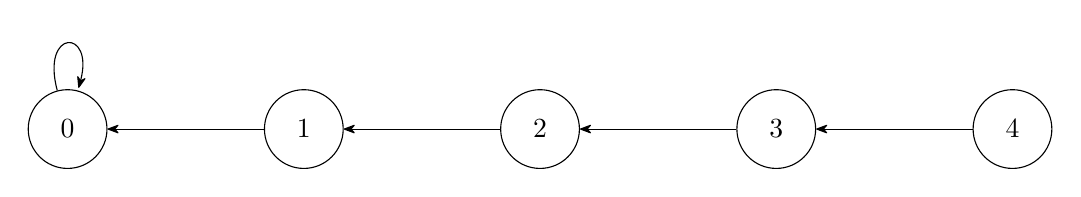
\begin{tikzpicture}[>={Stealth[round]}, node distance=2cm and 1cm, every node/.style={circle, draw, minimum size=1cm}]
    % Define vertices
    \node (v0) at (0, 0) {0};
    \node (v1) at (3, 0) {1};
    \node (v2) at (6, 0) {2};
    \node (v3) at (9, 0) {3};
    \node (v4) at (12, 0) {4};
    
    % Draw edges
    \draw [->] (v1) to (v0); % Edge 1 -> 0
    \draw [->] (v2) to (v1); % Edge 2 -> 1
    \draw [->] (v3) to (v2); % Edge 3 -> 2
    \draw [->] (v4) to (v3); % Edge 4 -> 3
    \draw[->] (v0) edge[loop above] (v0); % Self-loop at 0
\end{tikzpicture}
}
\end{center}
\ \\
\begin{center}   
$G_g: \;$
\resizebox{!}{3em}{
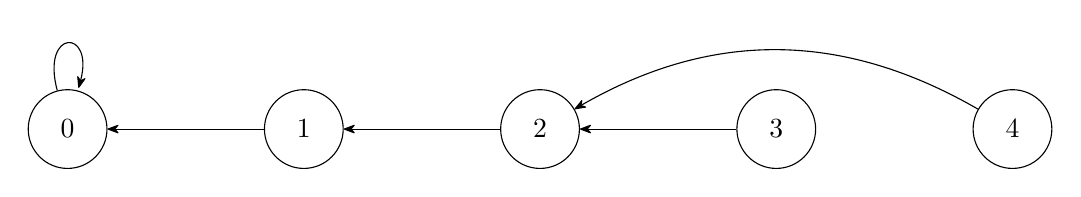
\begin{tikzpicture}[>={Stealth[round]}, node distance=2cm and 1cm, every node/.style={circle, draw, minimum size=1cm}]
    % Define vertices
    \node (v0) at (0, 0) {0};
    \node (v1) at (3, 0) {1};
    \node (v2) at (6, 0) {2};
    \node (v3) at (9, 0) {3};
    \node (v4) at (12, 0) {4};
    
    % Draw edges
    \draw [->] (v1) to (v0); % Edge 1 -> 0
    \draw [->] (v2) to (v1); % Edge 2 -> 1
    \draw [->] (v3) to (v2); % Edge 3 -> 2
    \draw [->] (v4) edge[bend right] (v2); % Edge 4 -> 2
    \draw[->] (v0) edge[loop above] (v0); % Self-loop at 0
\end{tikzpicture}
}
\end{center}

Run the SageMath script \texttt{ex1434.sage} to verify.
\end{example}

\bibliographystyle{alpha}
\bibliography{biblio}

\end{document}
